% SIAM Article Template
\documentclass[review,onefignum,onetabnum]{siamart190516}

% Information that is shared between the article and the supplement
% (title and author information, macros, packages, etc.) goes into
% ex_shared.tex. If there is no supplement, this file can be included
% directly.

% SIAM Shared Information Template
% This is information that is shared between the main document and any
% supplement. If no supplement is required, then this information can
% be included directly in the main document.


% Packages and macros go here
\usepackage{lipsum}
\usepackage{amsfonts}
\usepackage{graphicx}
\usepackage{epstopdf}
\usepackage{amsmath}
\usepackage{subcaption}
\usepackage{pgfplots}

%\usepackage{amsmath,amsthm}
%\usepackage[noend]{algorithmic}
%\usepackage{algorithmic}
\usepackage[algo2e, ruled, noend, linesnumbered]{algorithm2e}
%\usepackage[algo2e, ruled, vlined]{algorithm2e}
\usepackage{bm}
\ifpdf
  \DeclareGraphicsExtensions{.eps,.pdf,.png,.jpg}
\else
  \DeclareGraphicsExtensions{.eps}
\fi

\usepackage{placeins}
\usepackage{multirow}

% Add a serial/Oxford comma by default.
\newcommand{\creflastconjunction}{, and~}
\newcommand{\nor}[1]{\left\|#1\right\|}

% Used for creating new theorem and remark environments
\newsiamremark{remark}{Remark}
\newsiamremark{hypothesis}{Hypothesis}
\crefname{hypothesis}{Hypothesis}{Hypotheses}
\newsiamthm{claim}{Claim}
\newsiamthm{prop}{Proposition}
\newsiamthm{defn}{Definition}
\newsiamthm{thm}{Theorem}
\newsiamthm{cor}{Corollary}
\newsiamthm{lem}{Lemma}


\newcommand{\norm}[1]{\|#1\|}


% Sets running headers as well as PDF title and authors
\headers{Matrix-free PSF approximation}{N. Alger, T. Hartland, N. Petra, and O. Ghattas}

% Title. If the supplement option is on, then "Supplementary Material"
% is automatically inserted before the title.
\title{Matrix-free point spread function approximation of operators with locally supported non-negative integral kernels, with application to Hessians in PDE constrained inverse problems\thanks{Submitted to the editors DATE.
\funding{This research was supported by the National Science Foundation under Grant No. DMS-1840265 and CAREER-1654311.}}}

% Authors: full names plus addresses.
\author{Nick Alger\thanks{Oden Institute, The University of Texas at Austin, Austin, TX 
  (\email{nalger@oden.utexas.edu}).}
\and Tucker Hartland\thanks{Department of Applied Mathematics, University of California, Merced, Merced, CA. 
	(\email{thartland@ucmerced.edu}).}
\and Noemi Petra\thanks{Department of Applied Mathematics, University of California, Merced, Merced, CA. 
  (\email{npetra@ucmerced.edu}).}
\and Omar Ghattas\thanks{Oden Institute, The University of Texas at Austin, Austin, TX 
	(\email{omar@oden.utexas.edu}).}}

\newcommand{\Aop}{\mathcal{A}}
\newcommand{\AopPc}{\mathcal{A}_\text{pc}}
\newcommand{\AopPcMesh}{\mathcal{A}_\text{pc}^h}

\newcommand{\Aker}{\Phi}
\newcommand{\AkerPc}{\Phi_\text{pc}}
\newcommand{\AkerPcMesh}{\Phi_\text{pc}^h}

\newcommand{\AkerPcMat}{\mathbf{\Phi}_\text{pc}}

\newcommand{\Amat}{\mathbf{A}}
\newcommand{\AmatPc}{\mathbf{A}_\text{pc}}
\newcommand{\AmatPcSym}{\mathbf{A}_\text{pc}^\text{sym}}
\newcommand{\AmatPcSymPlus}{\mathbf{A}_\text{pc}^{\text{sym}+}}

\newcommand{\diraccomb}{\xi}
\newcommand{\combresponse}{\eta}
\newcommand{\weakadmconst}{C}
\newcommand{\horizinterpolant}{\theta}
\newcommand{\interpolatedvalues}{b}
\newcommand{\firstgreens}{G}
\newcommand{\secondgreens}{F}
\newcommand{\impulseresponse}{\phi}
\newcommand{\convkernel}{\varphi}
\newcommand{\febasis}{\psi}
\newcommand{\ratfct}{R}
\newcommand{\ratpole}{\omega}
\newcommand{\ratcoeff}{c}
\newcommand{\massmatrix}{\mathbf{M}}
\newcommand{\spatialvol}{V}
\newcommand{\spatialmean}{\mu}
\newcommand{\spatialcov}{\Sigma}
\newcommand{\genericdistribution}{\rho}
\newcommand{\pointbatch}{S}
\newcommand{\pointinteractionmatrix}{S}
\newcommand{\gdim}{d}
\newcommand{\fedim}{N}
\newcommand{\convrank}{r}
\newcommand{\hrank}{k_h}
\newcommand{\nbatch}{n_b}
\newcommand{\numnbr}{k_{n}}
\newcommand{\ratord}{l}
\newcommand{\nsamplepts}{m}
\newcommand{\ptsonebatch}{s}
\newcommand{\classicalrank}{r}
\newcommand{\secondgreenscoeff}{\beta}
\newcommand{\constcoeff}{\alpha}
\newcommand{\colcluster}{\mathtt{c}}
\newcommand{\rowcluster}{\mathtt{r}}
\newcommand{\icedomain}{U}
\newcommand{\basalfriction}{{q}}
\newcommand{\normalvec}{\nu}
\newcommand{\searchdir}{{\widehat{\basalfriction}}}
\newcommand{\preconditioner}{\widetilde{H}}
\newcommand{\candidatepts}{X}
\newcommand{\eigenvectormatrix}{P}
\newcommand{\candidatepoint}{x}
\newcommand{\velocity}{v}
\newcommand{\pressure}{p}
\newcommand{\rbfweight}{c}
\newcommand{\stress}{\sigma}
\newcommand{\tangentop}{T}
\newcommand{\strain}{\varepsilon}
\newcommand{\bodyforce}{f}
\newcommand{\observations}{y}
\newcommand{\rbf}{\varphi}
\newcommand{\fepoint}{\zeta}
\newcommand{\stokesrobincoeff}{{s}}
\newcommand{\regrobincoeff}{{s}}
\newcommand{\regrhs}{{f}}

\newcommand*{\vertbar}{\rule[-1ex]{0.5pt}{2.5ex}}
\newcommand*{\horzbar}{\rule[.5ex]{2.5ex}{0.5pt}}

\usepackage{amsopn}
\DeclareMathOperator{\diag}{diag}
\DeclareMathOperator{\interpolate}{Interpolate}
\DeclareMathOperator{\Span}{span}
\DeclareMathOperator{\Var}{Var}
\DeclareMathOperator{\vol}{vol}
\DeclareMathOperator{\avg}{avg}
\DeclareMathOperator*{\argmax}{arg\,max}
\DeclareMathOperator*{\argmin}{arg\,min}
\DeclareMathOperator{\dist}{dist}
\DeclareMathOperator{\diam}{diam}
\DeclareMathOperator{\nbrs}{nbrs}

\newcommand{\computediracresponse}[1]{\text{compute\_dirac\_comb\_response}\left( #1 \right)}
\newcommand{\ellipsoidsintersect}[2]{\text{ellipsoids\_intersect}\left( #1, #2 \right)}
\newcommand{\choosebatch}[1]{\text{choose\_sample\_point\_batch}\left( #1 \right)}
\newcommand{\computekernelentries}[2]{\text{compute\_approximate\_kernel\_entries}\left( #1 , #2 \right)}
\newcommand{\computeweightingentries}[1]{\text{compute\_weighting\_function\_entries}\left( #1 \right)}

\DeclareFontFamily{U}{wncy}{}
\DeclareFontShape{U}{wncy}{m}{n}{<->wncyr10}{}
\DeclareSymbolFont{mcy}{U}{wncy}{m}{n}
\DeclareMathSymbol{\Sh}{\mathord}{mcy}{"58} 

\SetEndCharOfAlgoLine{}
%\SetKwIF{If}{ElseIf}{Else}{if}{}{else if}{else}{end if}

%\renewcommand{\algorithmicrequire}{\textbf{Input:}}
%\renewcommand{\algorithmicensure}{\textbf{Output:}}


%%% Local Variables: 
%%% mode:latex
%%% TeX-master: "ex_article"
%%% End: 


% Optional PDF information
\ifpdf
\hypersetup{
  pdftitle={Fast matrix-free approximation of locally translation invariant operators that have locally supported non-negative integral kernels, with application to Hessians in PDE-constrained inverse problems},
  pdfauthor={N. Alger, N. Petra, T. Hartland, and O. Ghattas}
}
\fi

% The next statement enables references to information in the
% supplement. See the xr-hyperref package for details.

\externaldocument{localpsf_supplement}

% FundRef data to be entered by SIAM
%<funding-group specific-use="FundRef">
%<award-group>
%<funding-source>
%<named-content content-type="funder-name"> 
%</named-content> 
%<named-content content-type="funder-identifier"> 
%</named-content>
%</funding-source>
%<award-id> </award-id>
%</award-group>
%</funding-group>

\begin{document}

\maketitle

% REQUIRED
\begin{abstract}
	We present a fast matrix-free method for approximating operators that have locally supported non-negative integral kernels. Such operators arise, for example, as Schur complements in Schur complement methods for solving partial differential equations (PDEs), Poincare-Steklov operators in domain decomposition methods, covariance operators in spatial statistics, blurring operators in imaging, and Hessians in distributed parameter PDE-constrained inverse problems. Our method computes impulse responses of the operator at a collection of scattered points, then interpolates these known impulse responses to evaluate entries of the integral kernel at other points where the impulse response is not known. 
%	Classical H-matrix construction methods require access to matrix entries of the matrix being approximated, and therefore cannot be used to efficiently form H-matrix approximations of operators that are only available through matrix-vector products. 
	Impulse responses are computed by applying the operator to a small number of Dirac combs associated with ``batches'' of point sources. By solving an ellipsoid packing problem, we choose as many points as possible per batch, while ensuring that the supports of the impulse responses within each batch do not overlap. 
	The ability to rapidly evaluate kernel entries allows us to construct a hierarchical matrix (H-matrix) approximation of the operator. Fast H-matrix methods are used to perform further matrix computations including matrix-matrix addition and multiplication, matrix inversion and factorization, and matrix-vector products in nearly-linear complexity.
	We apply the method to approximate the Hessian in a large-scale PDE-constrained inverse problem with highly informative data. Numerical results demonstrate that our method substantially outperforms existing methods. We are able to approximate high rank operators using only a small number of operator applies.
\end{abstract}

% REQUIRED
\begin{keywords}
  
\end{keywords}

% REQUIRED
\begin{AMS}
  
\end{AMS}

\section{Introduction}
\label{sec:intro}

We present a fast \emph{matrix free} method for approximating operators, $\Aop:L^2(\Omega) \rightarrow L^2(\Omega)'$, that have locally supported non-negative integral kernels. Here $\Omega \subset \mathbb{R}^\gdim$ is a bounded domain, $\gdim$ is the spatial dimension, and $L^2(\Omega)'$ is the space of continuous linear functionals on $L^2(\Omega)$ (i.e., the topological dual space). Such operators arise as Schur complements in Schur complements methods for solving partial differential equations (PDEs) \cite{le1997non,saad1999distributed,TOBYPAPER}, Poincare-Steklov operators in domain decomposition methods (e.g., Dirichlet-to-Neumann maps) \cite{DTNMAP}, covariance operators in spatial statistics \cite{GeogaEtAl20,ChenStein21,LindgrenRueLindstrom11}, blurring operators in imaging \cite{DenisEtAl11,NagyOleary98}, and Hessians in distributed parameter PDE-constrained optimization and inverse problems \cite{AlgerEtAl19,IsaacEtAl15}. 

By ``matrix free,'' we mean that we have a black-box computational procedure through which we may apply $\Aop$ and its transpose\footnote{Recall that the transpose $\Aop^T:L^2(\Omega)\rightarrow L^2(\Omega)'$ is the unique operator satisfying $\left(\Aop u\right)(v) = \left(\Aop v\right)(u)$ for all $u,v \in L^2(\Omega)$, where the linear functional $\Aop u \in L^2(\Omega)'$ is the result of applying $\Aop$ to $u\in L^2(\Omega)$, the scalar $\left(\Aop u\right)(v)$ is the result of applying that linear functional to $v \in L^2(\Omega)$, and similar for the analogous operations with $\Aop^T$. }, $\Aop^T$, to arbitrary functions,
\begin{equation}
\label{eq:eval_maps}
u \mapsto\Aop u \qquad \text{and} \qquad v \mapsto \Aop^Tv,
\end{equation} 
but we do not have any further access to $\Aop$. In particular, we cannot easily access entries of $\Aop$'s integral kernel. In applications, evaluating the maps in \eqref{eq:eval_maps} may involve iteratively solving a large linear system, timestepping, or performing some other costly computational procedure. 

Our motivation is Hessian approximation in distributed parameter inverse problems governed by partial differential equations (PDEs). That is, inverse problems in which one seeks to reconstruct an unknown parameter field from noisy observations of a state variable that depends on the parameter implicitly through the solution of a PDE.
In the deterministic approach to the inverse problem, one solves a regularized minimization problem to find the parameter that best fits the data. The objective function in the minimization problem is defined implicitly, so information about the Hessian of the objective function is only accessible via application of the Hessian to vectors \cite{HESSIANACTION}. 
The most popular matrix-free Hessian approximation methods are based on low rank approximation \cite{BuiEtAl13,CuiEtAl14,FlathEtAl11,PetraEtAl14,SpantiniEtAl15} because there are efficient methods for constructing low rank approximations of a matrix using only matrix-vector products \cite{Cheng05,HalkoMartinssonTropp11}. 
However, low rank approximation methods suffer from a ``data predicament''---if the data are highly informative about the unknown parameter, then the numerical rank of the data misfit term in the Hessian is large, so a large number of operator applies are required to form an accurate ``low rank'' approximation \cite{Alger19,AlgerEtAl17}. High-rank approximation methods are needed.

\begin{figure}
	\begin{subfigure}{0.32\textwidth}
		\centering
		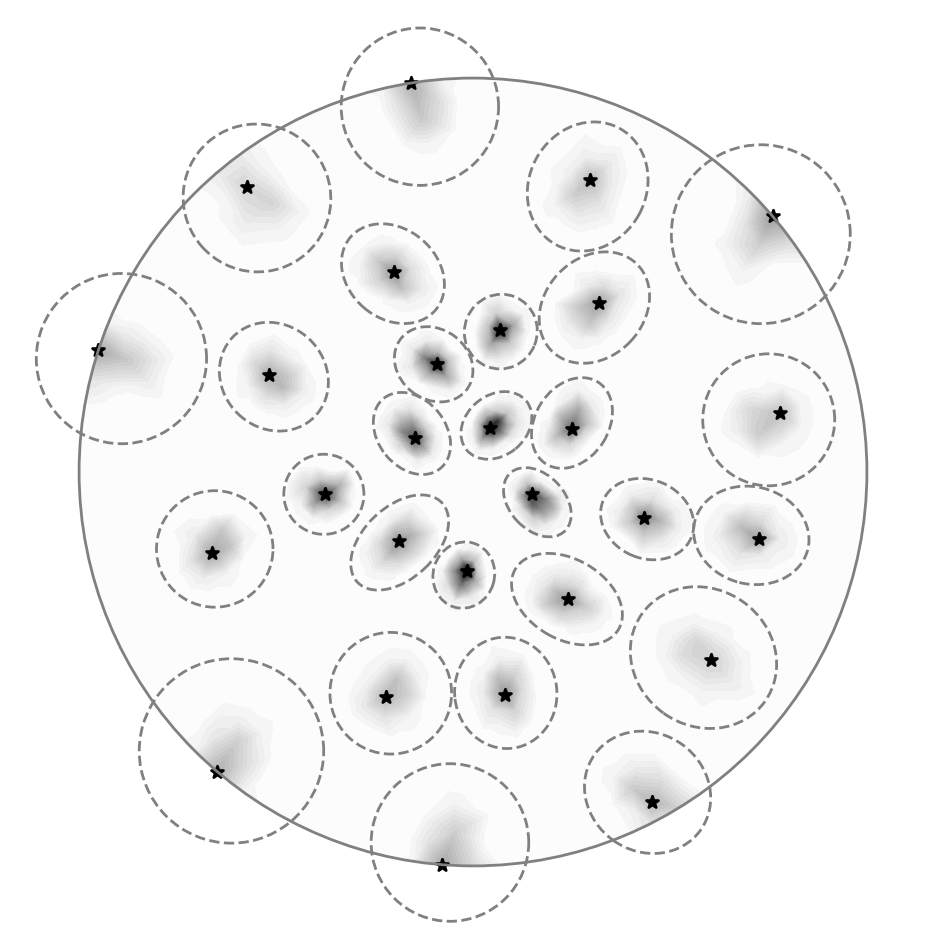
\includegraphics[scale=0.33]{impulse_batch1.png}
	\end{subfigure}
	\begin{subfigure}{0.32\textwidth}
		\centering
		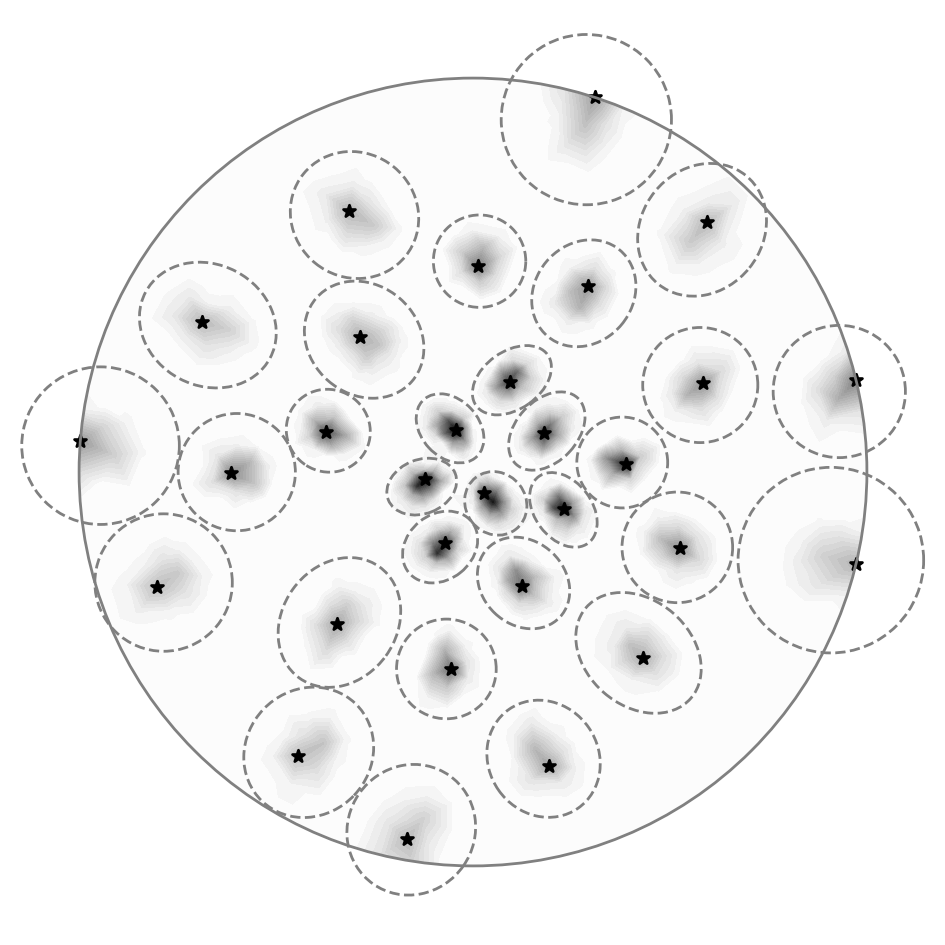
\includegraphics[scale=0.33]{impulse_batch2.png}
	\end{subfigure}
	\begin{subfigure}{0.32\textwidth}
		\centering
		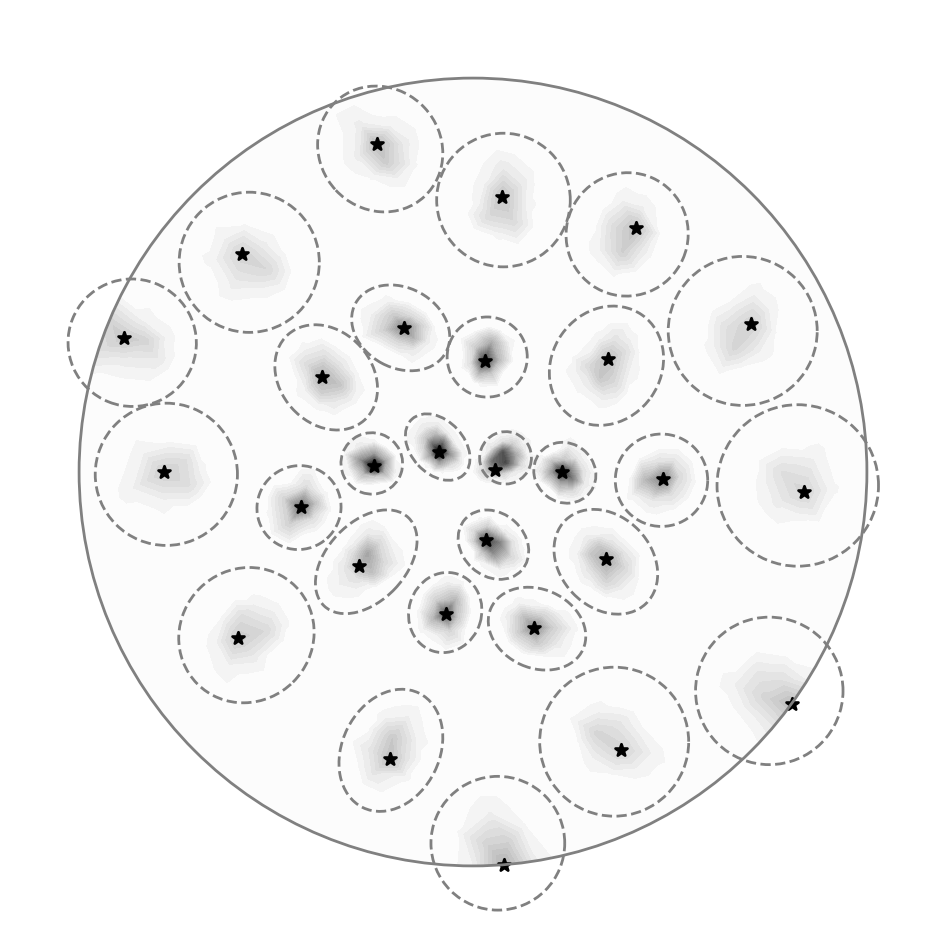
\includegraphics[scale=0.33]{impulse_batch3.png}
	\end{subfigure}
	\caption{Batches of normalized impulse responses for the Stokes inverse problem Hessian. 
%	Brightness scale differs between the subfigures. 
	Black stars indicate point source locations. Dashed gray ellipses indicate the estimated support ellipsoids. The large circle is the boundary of the domain. 
	}
	\label{fig:batches_intro}
\end{figure}

The central challenge we face is that existing scalable high-rank approximation methods typically require the ability to rapidly evaluate arbitrary entries of $\Aop$'s integral kernel, and we cannot do this because $\Aop$ is only accessible matrix-free. We address this challenge using \emph{impulse response interpolation}. The impulse response, $\phi_x$, associated with a point $x$ is the Riesz representation\footnote{Recall that the Riesz representative of a functional $\rho \in L^2(\Omega)'$ with respect to the $L^2$ inner product is the unique function $\rho^* \in L^2(\Omega)$ such that $\rho(v) = \left(\rho^*,v\right)_{L^2(\Omega)}$ for all $v \in L^2(\Omega)$.} of the linear functional that results from applying $\Aop$ to a delta distribution (i.e., point source, impulse) centered at $x$. We compute batches of impulse responses by applying $\Aop$ to weighted sums of delta distributions associated with batches of points scattered throughout the domain (see Figure \ref{fig:batches_intro}). Then we interpolate translated versions of these impulse responses to approximate arbitrary entries of the operator's integral kernel. 
%This allows fast evaluation of approximate matrix entries, which are needed by high-rank approximation methods, in particular, classical H-matrix construction methods. 

Picking the batches of points requires us to estimate the supports of the $\phi_x$, \emph{before} we compute them. The idea of estimating the supports of the functions $\phi_x$ a-priori was inspired by techniques from resolution analysis in seismic imaging, in which the width of $\phi_x$ is estimated to be the local autocorrelation length of the function $\Aop^T \zeta$ near $x$, where $\zeta$ is a random noise funtion  \cite{FichtnerLeeuwen15,TrampertFichtnerRitsema13}. Rather than probing $\Aop^T$ with random noise functions, we use polynomial functions (see Section \ref{sec:intromoments}). Our method estimates the support of $\phi_x$ more accurately and reliably than random noise probing at the cost of the additional constraint that $\Aop$ has a positive integral kernel.

Our impulse response interpolation procedure may be categorized as a ``point spread function'' (PSF) method that is loosely based on so-called ``product-convolution'' (PC) approximations, which are approximations of an operator by weighted sums of convolution operators with spatially varying weights. PC and PSF methods have a long history dating back several decades. We note the following papers (among many others),  \cite{Adorf94,AlgerEtAl19,BigotEscandeWeiss19,NagyOleary98,FishEtAl96,EscandeWeiss12,EscandeWeiss15,EscandeWeiss22,ZhuLiFomelEtAl16}, in which the convolution kernels are constructed from sampling impulse responses of the operator to scattered point sources. For background on PC and PSF methods, we recommend the following papers which provide well-written reviews of the topic: \cite{DenisEtAl15,EscandeWeiss17,GentileCourbinMeylan13}. While PC approximations are based on an assumption of local translation invariance, the method we propose is based on an assumption that we call ``local mean displacement invariance'' (see Figure \ref{fig:mean_displacement_invariance}). This is more general than local translation invariance, and includes both low rank approximation and local translation invariance as special cases (see Section \ref{sec:local_mean_displacement_invariance}). Furthermore, PC approximations have well-known issues near boundaries due to so-called ``boundary artifacts,'' caused by the boundary artificially ``cutting off'' impulse responses. We avoid this issue by temporarily excluding impulse responses from the approximation procedure whenever an attempt is made to evaluate the impulse response at a location where it is undefined. 

%\begin{figure}
%	\begin{center}
%		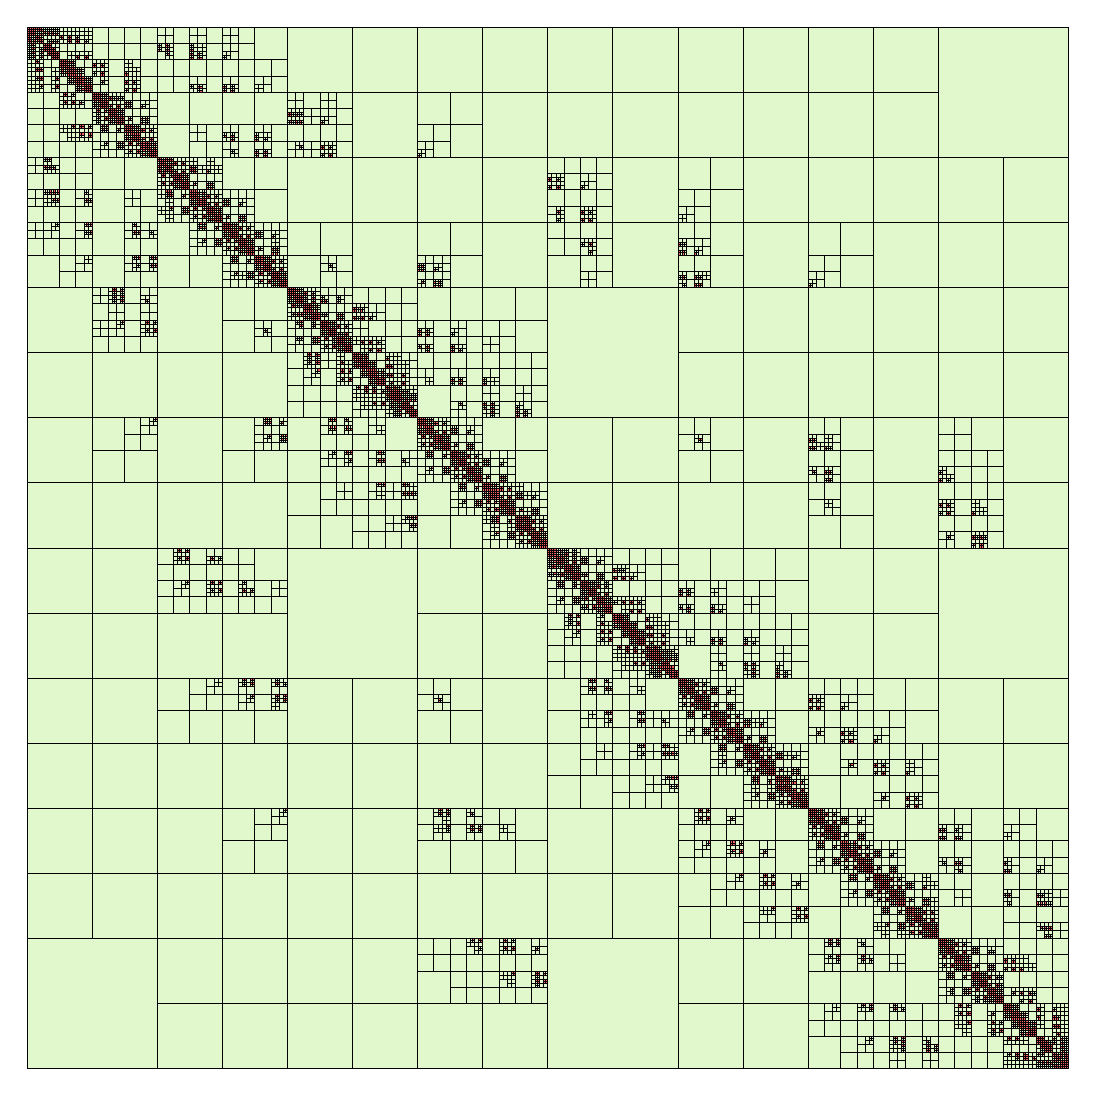
\includegraphics[scale=0.4]{bct1.eps}
%	\end{center}
%	\caption{Hierarchical matrix block structure for the Stokes Hessian. The red blocks (tiny) are dense. All other blocks are low rank.
%	}
%	\label{fig:hmatrix_intro}
%\end{figure}

The ability to rapidly evaluate approximations of arbitrary entries of $\Aop$'s integral kernel allows us to form a hierarchical matrix (H-matrix) \cite{Hackbusch99,} approximation of a discretized version of $\Aop$. H-matrices are a matrix format in which the rows and columns of the matrix are re-ordered, then the matrix is recursively subdivided into blocks, in such a way that many off-diagonal blocks are low rank, even though the matrix as a whole may be high-rank. 
%(see Figure \ref{fig:hmatrix_intro} and Appendix \ref{app:h_matrix}).
H-matrix methods permit us to perform matrix-vector products cheaply. Furthermore, one may use H-matrix methods to perform useful linear algebra operations involving the H-matrix that cannot easily be done using the original operator. These operations include matrix-matrix addition, matrix-matrix multiplication, matrix factorization, and matrix inversion. 
%These H-matrix methods are fast and scale well to large problems. 
The work and memory required to perform these operations for an $\fedim \times \fedim$ H-matrix is scales as $O(\fedim \log(\fedim)^a)$, where $a \in \{0,1,2,3\}$. That is, the cost is \emph{nearly-linear} in $N$. The exact cost depends on the type of H-matrix used, the operation being performed, and the rank of the off-diagonal blocks; for more details see \cite{GrasedyckHackbusch03}. The ability to perform these operations permits, for example, fast solution of Newton linear systems in PDE-constrained optimization, fast sampling of ill-conditioned posterior distribution in Bayesian inverse problems, and construction of high rank surrogate models that can be used for uncertainty quantification. 

%Classical H-matrix construction methods 
%(described in Appendix \ref{sec:H_matrix_construction}) 
%require access to matrix entries of the matrix being approximated, and therefore cannot be used to efficiently form H-matrix approximations of operators that are only available matrix free.
Recently there have been improvements in matrix-free H-matrix construction methods based on the so-called ``peeling process'' \cite{LinYing11,Martinsson11,Martinsson16,MartinssonTropp20}, which we do not use here. 
These alternative methods have been applied to form H-matrix representations of Hessians in PDE constrained inverse problems \cite{AmbartsumyanEtAl20,HartlandEtAl22}. 
Methods based on the peeling process are asymptotically scalable (typically the number of matrix vector products required scales as $O(\log N)$), but in practice the required number of matrix vector products is large. Improving the peeling process to reduce its cost is currently an area of active research \cite{PEELINGRESEARCH}.
%This is an area of active research, so more efficient and practical matrix-free H-matrix construction methods based on the peeling process may be discovered in the future.
%Matrix-free H-matrix construction methods are currently a topic of considerable research, so more efficient matrix-free H-matrix methods based on the peeling process may be discovered in the future. 



\begin{figure}
	\begin{center}
		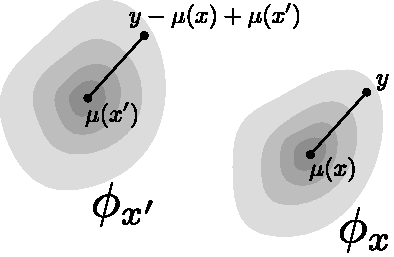
\includegraphics[scale=1.0]{mean_displacement_invariance.pdf}
	\end{center}
	\caption{An operator is locally mean-displacement invariant if $\impulseresponse_{x}(y) \approx \impulseresponse_{x'}\left(y - \spatialmean(x) + \spatialmean(x')\right)$ when $x$ is close to $x'$. Here $\spatialmean(x)$ is the mean (center of mass) of $\phi_x$, and similar for $\spatialmean(x')$.}
	\label{fig:mean_displacement_invariance}
\end{figure}


\section{Preliminaries}

Let $\Omega \subset \mathbb{R}^\gdim$ be a bounded domain (in applications typically $\gdim=1$, $2$, or $3$). We seek to approximate integral operators $\Aop:L^2(\Omega)\rightarrow L^2(\Omega)'$ that may be written in the following form:
\begin{equation}
\label{eq:kernel_representation}
(\Aop u)(v) := \int_\Omega \int_\Omega v(y) \Aker(y,x) u(x) dx dy.
\end{equation}
Here the linear functional $\Aop u \in L^2(\Omega)'$ is the result of applying $\Aop$ to $u\in L^2(\Omega)$, the scalar $\left(\Aop u\right)(v)$ is the result of applying that linear functional to $v \in L^2(\Omega)$.
The function $\Aker:\Omega \times \Omega \rightarrow \mathbb{R}$ is the integral kernel, which exists in principle but is not easily accessible to us. In this section we describe how to extend the action of $\Aop$ to distributions, which allows us to define the impulse responses (Section \ref{sec:impulse_response_2}). Then we state the conditions on $\Aop$ that our method requires (Section \ref{sec:conditions_2}). Finally, we detail finite element discretization (Section \ref{sec:finite_element_kernel}).


\subsection{Distributions and impulse responses}
\label{sec:impulse_response_2}

The action of $\Aop$ may be extended to distributions if the kernel $\Aker$ is sufficiently regular. We derive the extension as follows. Suppose $\rho \in L^2(\Omega)'$, and let $\rho^* \in L^2(\Omega)$ denote the Riesz representative of $\rho$ with respect to the $L^2(\Omega)$ inner product. We have
\begin{subequations}
	\label{eq:extension_to_distributions}
	\begin{align}
		\left(\Aop \genericdistribution^*\right)(v) &= \int_\Omega \int_\Omega v(y) \Aker(y,x) \genericdistribution^*(x) dx ~dy \\
		&= \int_\Omega v(y) \int_\Omega \Aker(y,x) \genericdistribution^*(x) dx ~dy \\
		&= \int_\Omega v(y) \genericdistribution\left(\Aker(y,\cdot)\right) dy, \label{eq:action_on_distribution}
	\end{align}
\end{subequations}
where $\Aker(y,\cdot)$ denotes the function $x \mapsto \Aker(y,x)$.
Now let $\mathcal{D}(\Omega) \subset L^2(\Omega)$ be a suitable space of test functions, and instead suppose $\rho:\mathcal{D}(\Omega) \rightarrow \mathbb{R}$ is a distribution. In this case, the Riesz representative $\rho^*$ may not exist, so the derivation in \eqref{eq:extension_to_distributions} is not valid. However, if $\Aker$ is sufficiently regular such that the function $y \mapsto \rho\left(\Aker(y,~\cdot~)\right)$ is well-defined for almost all $y\in\Omega$, and if this function is in $L^2(\Omega)$, then the right hand side of \eqref{eq:action_on_distribution} is well-defined. Hence, we \emph{define} the action of $\Aop$ on the distribution $\rho$ to be the right hand side of \eqref{eq:action_on_distribution}. For convenience of notation, we denote this action by ``$\Aop \genericdistribution^*$,'' even if $\rho^*$ does not exist.

Let $\delta_x$ denote the delta distribution\footnote{Recall that the delta distribution $\delta_x:\mathcal{D}(\Omega)\rightarrow \mathbb{R}$ is the linear functional defined by $\delta_x(v) = v(x)$ for all $v\in \mathcal{D}(\Omega)$.} (i.e., point source, impulse) centered at the point $x \in \Omega$.
The \emph{impulse response} of $\Aop$ associated with $x$ is the function $\impulseresponse_x:\Omega \rightarrow \mathbb{R}$, 
\begin{equation}
\label{eq:impulse_response_delta_action}
\impulseresponse_x := \left( \Aop \delta_x^* \right)^*,
\end{equation}
that is formed by applying $\Aop$ to $\delta_x$, then taking the Riesz representation of the resulting linear functional. Using \eqref{eq:action_on_distribution} and the definition of the delta distribution, we see that $\phi_x$ may also be written as the function
\begin{equation}
\label{eq:impulse_response_defn}
\impulseresponse_x(y) = \Aker(y, x),
\end{equation} 
which results from keeping $x$ fixed and viewing $\Aker(y,x)$ as a function of $y$. 

\subsection{Required conditions}
\label{sec:conditions_2}

We focus on approximating operators that satisfy the following conditions: 
\begin{enumerate}
	\item The kernel $\Aker$ is sufficiently regular such that $\phi_x$ is a well-defined function for all $x\in \Omega$.
	\item The supports of the impulse responses $\impulseresponse_x$ are contained in localized regions.
	\item The integral kernel is non-negative in the sense that $$\Aker(y,x) \ge 0$$ for all $(y,x) \in \Omega \times \Omega$.\footnote{Note that having a non-negative integral kernel is different from positive semi-definiteness. The operator $\Aop$ need not be positive semi-definite to use our method, and positive semi-definite operators need not have a non-negative integral kernel.}
\end{enumerate}
Our method may still perform well if these conditions are relaxed slightly. For example, it is fine if the support of the impulse response $\impulseresponse_x$ is not perfectly contained in a localized region, so long as the bulk of the ``mass'' of the impulse response is contained in a localized region. The integral kernel does not need to be non-negative for all pairs of points $(y,x) \in \Omega \times \Omega$, as long as it is non-negative for the vast majority of pairs of points $(y,x)$, and as long as the negative numbers are comparatively small. If these conditions are violated, our method will incur additional error. If these conditions are violated too much, our method may fail. Not all operators of interest (and in particular not all Hessians) satisfy these conditions, but many operators of practical interest do satisfy these conditions, and our method is highly effective for approximating these operators.

\subsection{Finite element discretization}
\label{sec:finite_element_kernel}

In computations, functions are discretized and replaced by finite dimensional vectors, and operators mapping between infinite dimensional spaces are replaced by operators mapping between finite dimensional spaces. In this paper we discretize using continuous Galerkin finite elements satisfying the Kronecker property (defined below). With minor modifications, our method could be used with more general finite element methods, or other discretization schemes such as finite differences or finite volumes.

Let $\febasis_1, \febasis_2, \dots, \febasis_\fedim$ be a set of continuous Galerkin finite element basis functions used to discretize the problem on a mesh with mesh size parameter $h$, let $V_h := \Span\left(\febasis_1, \febasis_2, \dots, \febasis_\fedim\right)$ be the corresponding finite element space under the $L^2$ inner product, and let $p_i \in \mathbb{R}^\gdim$, $i=1,\dots, \fedim$ be the Lagrange nodes associated with the functions $\febasis_i$. We assume that the finite element basis satisfies the Kronecker property, i.e., $\febasis_i(p_i)=1$ and $\febasis_i(p_j)=0$ if $i\neq j$. 
For $u_h \in V_h$ we write $\bm{u} \in \mathbb{R}^\nsamplepts_\massmatrix$ to denote the coefficient vector for $u_h$ with respect to the finite element basis, i.e.,
\begin{equation}
\label{eq:fem_coeff_basis}
u_h(x) = \sum_{i=1}^\fedim \bm{u}_i \febasis_i(x).
\end{equation}
Linear functionals $\rho_h \in V_h'$ have coefficient dual vectors $\boldsymbol{\rho}\in \mathbb{R}^\nsamplepts_{\massmatrix^{-1}}$, with entries 
\begin{equation*}
\boldsymbol{\rho}_i = \rho_h(\febasis_i), \qquad i=1,\dots,\nsamplepts. 
\end{equation*}
Here $\massmatrix \in \mathbb{R}^{\fedim \times \fedim}$ denotes the sparse finite element mass matrix which has entries
\begin{equation*}
\massmatrix_{ij}=\int_\Omega \febasis_i(x) \febasis_j(x) dx, \qquad i,j=1,\dots,\fedim,
\end{equation*}
the space $\mathbb{R}^\fedim_\massmatrix$ is $\mathbb{R}^\fedim$ with the inner product $(\mathbf{u},\mathbf{v})_\massmatrix := \mathbf{u}^T \massmatrix \mathbf{v}$, and $\mathbb{R}^\fedim_{\massmatrix^{-1}}$ is the analogous space with $\massmatrix^{-1}$ replacing $\massmatrix$. Direct calculation shows that $\mathbb{R}^\fedim_\massmatrix$ and $\mathbb{R}^\fedim_{\massmatrix^{-1}}$ are isomorphic to $V_h$ and $V_h'$ as Hilbert spaces, respectively.

After discretization, the operator $\Aop:L^2(\Omega) \rightarrow L^2(\Omega)'$ is replaced by an operator $A_h:V_h \rightarrow V_h'$, which becomes an operator
\begin{equation*}
\mathbf{A}:\mathbb{R}^\fedim_\massmatrix \rightarrow \mathbb{R}^\fedim_{\massmatrix^{-1}}
\end{equation*}
under the isomorphism discussed above. Our method is agnostic to the computational procedure for approximating $\Aop$ with $\mathbf{A}$. What is important is that we do not have direct access to matrix entries $\mathbf{A}_{ij}$. Rather, we have a computational procedure that allows us to compute matrix-vector products $\mathbf{u}\mapsto \mathbf{A}\mathbf{u}$ and $\mathbf{v}\mapsto \mathbf{A}^T\mathbf{v}$, and computing these matrix-vector products is costly.
Of course, matrix entries can be computed via matrix-vector products as $\mathbf{A}_{ij} = \left(\mathbf{A}\mathbf{e}_j\right)_i$,
where $\mathbf{e}_j=(0,\dots,0,1,0,\dots,0)^T$ is the length $\fedim$ unit vector with one in the $j$th coordinate and zeros elsewhere. But computing the matrix-vector product $\mathbf{e}_j \mapsto \mathbf{A}\mathbf{e}_j$ is costly, and therefore wasteful if we do not use other matrix entries in the $j$th column of $\mathbf{A}$. Hence, methods for approximating $\mathbf{A}$ are computationally intractable if they require accessing scattered matrix entries from many different rows and columns of $\mathbf{A}$. 

The operator $A_h:V_h \rightarrow V_h'$ can be written in integral kernel form as
\begin{equation}
(A_h u_h)(v_h) := \int_\Omega \int_\Omega v_h(y) \Aker_h(y,x) u_h(x) dx dy
\end{equation}
for some kernel $\Aker_h$ which we do not know, and which may differ from $\Aker$ due to discretization error. Since the functions in $V_h$ are continuous at $x$, the delta distribution $\delta_x$ is a continuous linear functional on $V_h$, which has a discrete dual vector $\boldsymbol{\delta}_x \in \mathbb{R}^\fedim_{\massmatrix^{-1}}$ with entries $\left(\boldsymbol{\delta}_x\right)_i = \febasis_i(x)$ for $i=1,\dots,\fedim$. Additionally, it is straightforward to verify that the Riesz representation, $\rho_h^* \in V_h$, of a functional $\rho \in V_h'$ has coefficient vector
\begin{equation*}
\boldsymbol{\rho}^* = \massmatrix^{-1} \boldsymbol{\rho}.
\end{equation*}
Therefore, the formula for the impulse response from \eqref{eq:impulse_response_delta_action} becomes 
\begin{equation}
\label{eq:discrete_kernel}
\boldsymbol{\impulseresponse}_x = \left(A_h \delta_x^*\right)^* =  \massmatrix^{-1}\mathbf{A} \massmatrix^{-1} \boldsymbol{\delta}_x,
\end{equation}
and the $(y,x)$ kernel entry of $\Aker_h$ may be written as
\begin{equation}
\label{eq:approx_kernel_entry_81}
	\Aker_h(y,x) = \boldsymbol{\delta}_y^T \boldsymbol{\impulseresponse}_x = \boldsymbol{\delta}_y^T \massmatrix^{-1}\mathbf{A} \massmatrix^{-1} \boldsymbol{\delta}_x.
\end{equation}
Now define $\mathbf{\Aker} \in \mathbb{R}^{\fedim \times \fedim}$ to be the following dense matrix of kernel entries evaluated at all pairs of Lagrange nodes:
\begin{equation}
\label{eq:Akerpcmat_entries}
\mathbf{\Aker}_{ij} := \Aker_h(p_i, p_j).
\end{equation}
Because of the Kronecker property of the finite element basis, we have $\boldsymbol{\delta}_{p_i} = \mathbf{e}_i$. Thus from \eqref{eq:approx_kernel_entry_81} we have
$
	\Aker_h(p_i,p_j) = \left(\massmatrix^{-1}\mathbf{A} \massmatrix^{-1}\right)_{ij},
$
which implies
\begin{equation}
\label{eq:boldA}
	\mathbf{A} = \massmatrix \mathbf{\Aker} \massmatrix.
\end{equation}
Broadly, our method will construct an H-matrix approximation of $\mathbf{A}$ by forming H-matrix approximations of $\boldsymbol{\Aker}$ and $\massmatrix$ (or a lumped mass version of $\massmatrix$), then multiplying these matrices with H-matrix methods per \eqref{eq:boldA}. The central challenge is that classical H-matrix construction methods require access to arbitrary matrix entries $\mathbf{\Aker}_{ij}$, but these matrix entries are not easily accessible. The bulk of our method is therefore dedicated to forming approximations of these matrix entries that can be evaluated rapidly.

\paragraph{Lumped mass matrix} At the continuum level, the integral kernel $\Aker$ is assumed to be non-negative. However, when we compute impulse responses we are effectively operating with the discrete integral kernel shown in \eqref{eq:approx_kernel_entry_81}.
The inverse mass matrices in this formula, $\massmatrix^{-1}$, will typically contain negative numbers. If there are too many negative numbers, or if the negative numbers are too large, our algorithm will be less robust. We therefore recommend replacing the mass matrix $\massmatrix$ with a positive diagonal \emph{lumped mass} approximation. 
In our numerical results, we use the lumped mass matrix constructed by replacing off-diagonal entries of the mass matrix by zero. Other more advanced mass lumping techniques may be used. See \cite{Hughes12} for a discussion of lumped mass matrices.


\section{Key innovations}
\label{sec:prerequisites}

In this section we present two key innovations that our method is based on.
First, we define moments of the impulse responses, $\phi_x$, show how these moments can be computed efficiently, and use these moments to form ellipsoid shaped a-priori estimates for the supports of the impulse responses (Section \ref{sec:intromoments}). Our method will use these ellipsoid estimates to choose sets of impulse responses that can be computed in batches. Second, we describe an improved method of approximating impulse responses by other nearby impulse responses, which we call ``normalized local mean displacement invariance'' (Section \ref{sec:local_mean_displacement_invariance}). Our method will interpolate impulse responses using this approximation. 



\subsection{Impulse response moments and ellipsoid support estimate}
\label{sec:intromoments}

The impulse response $\impulseresponse_x$ may be interpreted as a scaled probability distribution because of the non-negative integral kernel property. Let $\spatialvol:\Omega \rightarrow \mathbb{R}$,
\begin{equation}
\label{eq:define_vol}
\spatialvol(x) := \int_\Omega \impulseresponse_x(y) dy
\end{equation}
denote the spatially varying scaling factor, and for $i,j=1,\dots,\gdim$ define $\spatialmean:\Omega \rightarrow \mathbb{R}^\gdim$ and $\spatialcov:\Omega \rightarrow \mathbb{R}^{\gdim \times \gdim}$ as follows:
\begin{align}
\spatialmean^i(x) :=& \int_\Omega (\impulseresponse_p(y) / V(x)) y^i ~dy \label{eq:define_mean} \\
\spatialcov^{ij}(x) :=& \int_\Omega (\impulseresponse_p(y) / V(x)) \left(y^i - \spatialmean^i(x)\right) \left(y^j - \spatialmean^j(x)\right) ~dy, \label{eq:define_cov}
\end{align}
where $\spatialmean^i(x)$ denotes the $i^\text{th}$ component of the vector $\spatialmean(x)$, and $\spatialcov^{ij}(x)$ denotes the $(i,j)$ entry of the matrix $\spatialcov(x)$.
The vector $\spatialmean(x)\in \mathbb{R}^\gdim$ and the matrix $\spatialcov(x) \in \mathbb{R}^{\gdim \times \gdim}$ are the mean and covariance of the normalized version of $\impulseresponse_x$, respectively. 

The direct approach to compute $\spatialvol(x)$, $\spatialmean(x)$, and $\spatialcov(x)$ is to apply $\Aop$ to a point source centered at $x$ to obtain $\impulseresponse_x$, as per \eqref{eq:impulse_response_delta_action}. Then one can post-process $\impulseresponse_x$ to determine $\spatialvol(x)$, $\spatialmean(x)$, and $\spatialcov(x)$. However, this direct approach is not feasible because we need to know $V(x)$, $\spatialmean(x)$, and $\spatialcov(x)$ before we compute $\phi_x$, in order choose the point $x$. Computing $\phi_x$ in order to determine $V(x)$, $\spatialmean(x)$, and $\spatialcov(x)$ would be extremely computationally expensive, and defeat the purpose of our algorithm, which is to reduce the computational cost by computing impulse responses in batches. Fortunately, it is possible to compute $\spatialvol(x)$, $\spatialmean(x)$, and $\spatialcov(x)$ indirectly, \emph{for all points $x\in\Omega$ simultaneously}, by applying $\Aop^T$ to one constant function, $\gdim$ linear functions, and $\gdim(\gdim+1)/2$ quadratic functions (e.g., 6 total operator applies in two spatial dimensions and 10 in three spatial dimensions). This may be motivated by analogy to matrices. If $\mathbf{B}\in \mathbb{R}^{\fedim \times \fedim}$ is a matrix with $i^\text{th}$ column $\mathbf{b}_i$ and $\mathbf{f} \in \mathbb{R}^\fedim$, then
\begin{equation*}
\mathbf{B}^T \mathbf{f} = \begin{bmatrix}
\horzbar & \mathbf{b}_1^T & \horzbar \\
\horzbar & \mathbf{b}_2^T & \horzbar \\
& \vdots & \\
\horzbar & \mathbf{b}_\fedim^T & \horzbar
\end{bmatrix}
\mathbf{f} = 
\begin{bmatrix}
\mathbf{b}_1^T \mathbf{f} \\
\mathbf{b}_2^T \mathbf{f} \\
\vdots \\
\mathbf{b}_\fedim^T \mathbf{f}
\end{bmatrix}.
\end{equation*}
By computing one matrix-vector product of $\mathbf{B}^T$ with $\mathbf{f}$, we compute the inner product of each column of $\mathbf{B}$ with $\mathbf{f}$ simultaneously. The operator case is analogous, with the impulse response $\phi_x$ taking the place of a matrix column. We have
\begin{equation}
\label{eq:operator_simultaneous_ips}
\left(\Aop^T f\right)^*(x) = \int_\Omega \Aker(y,x) f(y) dy = \left(\phi_x, f\right)_{L^2(\Omega)}.
\end{equation}
By computing one operator application of $\Aop^T$ to $f$, we compute the inner product of each impulse response $\phi_x$ with $f$, for all points $x$ simultaneously. 

Let $C$, $L^i$, and $Q^{ij}$ be the following constant, linear, and quadratic functions:
\begin{equation*}
C(x) := 1, \qquad
L^i(x) := x^i, \qquad
Q^{ij}(x) := x^i x^j
\end{equation*}
for $i,j=1,\dots,\gdim$. Using the definition of $\spatialvol$ in \eqref{eq:define_vol} and using \eqref{eq:operator_simultaneous_ips}, we have
\begin{equation*}
	\spatialvol(x) = \int_\Omega \phi_x(y) C(y) ~ dy = \left(\phi_x, C\right)_{L^2(\Omega)} = \left(\mathcal{A}^T C\right)^*(x).
\end{equation*}
Hence, we may compute $\spatialvol(x)$ for all $x$ simultaneously by applying $\Aop^T$ to $C$. Analogous manipulations show that $\spatialmean(x)$ and $\spatialcov(x)$ may be computed for all points $x$ simultaneously by applying $\Aop^T$ to the functions $L^i$ and $Q^{ij}$, respectively. To summarize the results of doing this, we have
\begin{subequations}
	\label{eq:vol_mean_var}
	\begin{align}
	\spatialvol =& \left(\Aop^T C\right)^* \\
	\spatialmean^i =& \left(\Aop^T L^i\right)^* / \spatialvol \\
	\spatialcov^{ij} =& \left(\Aop^T Q^{ij}\right)^* / \spatialvol - \spatialmean^i\cdot \spatialmean^j
	\end{align}
\end{subequations}
for $i,j=1,\dots, \gdim$. Here $f/g$ denotes pointwise division of functions, $\left(f/g\right)(x) = f(x)/g(x)$, and $f\cdot g$ denotes pointwise multiplication of functions, $(f\cdot g)(x) = f(x)g(x)$.
%The resulting method for computing discretized versions of $\spatialvol$, $\spatialmean$, and $\spatialcov$ is shown in Algorithm \ref{alg:varhpi_mean_cov}.

%\begin{algorithm2e}
%	\SetAlgoNoLine
%	\SetKwInOut{Input}{Input}
%	\SetKwInOut{Output}{Output}
%	{	
%		\Input{Operator $\bm{A}^T$}
%		\Output{$\bm{\spatialvol}\in \mathbb{R}^\fedim$, $\bm{\spatialmean}\in \mathbb{R}^{\gdim \times \fedim}$, and $\bm{\spatialcov} \in \mathbb{R}^{\gdim \times \gdim \times \fedim}$}
%		
%		Form vector $\bm{C} \in \mathbb{R}^\fedim_{\massmatrix}$ by either projecting or interpolating constant function $C(x)=1$ onto $V_h$
%		
%		$\bm{\spatialvol} \gets \massmatrix^{-1}\bm{A}^T \bm{C}$
%		
%		\For{$i=1,2,\dots,\gdim$}{
%			Form vector $\bm{L}^i \in \mathbb{R}^\fedim_{\massmatrix}$ by either projecting or interpolating linear function $L^i(x) = x^i$ onto $V_h$
%			
%			$\bm{\spatialmean}^i \gets \left(\massmatrix^{-1}\bm{A}^T \bm{L}^i\right) / \bm{\spatialvol}$
%		}
%		\For{$i=1,2,\dots,\gdim$}{
%			\For{$j=1,\dots,i$}{
%				Form quadratic function $\bm{Q}^{ij} = x^i x^j$
%				
%				$\bm{\spatialcov}^{ij} \gets \left(\massmatrix^{-1}\bm{A}^T \bm{Q}^{ij}\right) / \bm{\spatialvol} - \bm{\spatialmean}^i\cdot \bm{\spatialmean}^j$
%				
%				$\bm{\spatialcov}^{ji} \gets \bm{\spatialcov}^{ij}$
%				
%			}
%		}
%		
%	}
%	\caption{Compute discretized scaling factor $\mathbf{\spatialvol}$, mean $\boldsymbol{\spatialmean}$, and covariance $\boldsymbol{\spatialcov}$}
%	\label{alg:varhpi_mean_cov}
%\end{algorithm2e}

Next, we make the approximation that the support of $\impulseresponse_x$ is contained within the ellipsoid
\begin{equation}
\label{eq:support_ellipsoid}
E_x := \{x' \in \Omega: (x' - \spatialmean(x))^T \spatialcov(x)^{-1} (x' - \spatialmean(x)) \le \tau^2\},
\end{equation}
where $\tau$ is a fixed constant. The ellipsoid $E_x$ is the set of points within $\tau$ standard deviations from the mean of the Gaussian distribution with mean $\spatialmean(x)$ and covariance $\spatialcov(x)$, i.e., the Gaussian distribution which has the same mean and covariance as the normalized version of $\impulseresponse_x$.

The quantity $\tau$ is a parameter that must be chosen appropriately. The larger $\tau$ is, the larger the ellipsoid $E_x$ is, and the more conservative the estimate is for the support of $\impulseresponse_x$. However, in Section \ref{sec:sample_point_selection} we will see that the cost of our algorithm depends on how many non-overlapping ellipsoids $E_x$ we can ``pack'' in the domain $\Omega$ (the more ellipsoids the better), and choosing a larger value of $\tau$ means that fewer ellipsoids will fit in $\Omega$. In practice, we find that $\tau=3$ yields a reasonable balance between these competing interests, and use $\tau=3$ in our numerical results. The fraction of the ``mass'' of $\impulseresponse_x$ residing outside of $E_x$ is less than $1/\tau^2$ by Chebyshev's inequality, though this bound is conservative and typically far less mass resides in this region. 


\subsection{Local mean-displacement invariance}
\label{sec:local_mean_displacement_invariance}

Let $x$ and $x'$ be points in $\Omega$ that are ``close'' to each other, and consider the following approximations:
\begin{align}
\phi_x(y) &\approx \phi_{x'}(y) \label{eq:translate1}\\
\phi_x(y) &\approx \phi_{x'}(y-x+x') \label{eq:translate2}\\
\phi_x(y) &\approx \phi_{x'}\left(y-\spatialmean(x)+\spatialmean(x')\right) \label{eq:translate3}\\
\phi_x(y)/\spatialvol(x) &\approx \phi_{x'}\left(y-\spatialmean(x)+\spatialmean(x')\right) / \spatialvol(x'). \label{eq:translate4}
\end{align}
These are four different ways to approximate an impulse response by a nearby impulse response, with each successive approximation building upon the previous ones. Our method uses \eqref{eq:translate4}, which is the most sophisticated of these approximations.

Approximation \eqref{eq:translate1} says that $\phi_x$ can be approximated by $\phi_{x'}$ when $x$ and $x'$ are close. Operators satisfying \eqref{eq:translate1} can be well-approximated via low-rank CUR approximation \cite{CUR,NYSTROM}. However, the required rank in the low rank approximation can be large, which makes algorithms based on \eqref{eq:translate1} expensive. 

Operators that satisfy \eqref{eq:translate2} are called ``locally translation-invariant'' because integral kernel entries $\Aker(y,x)$ for such operators are approximately invariant under translation of $x$ and $y$ by the same displacement, i.e., $x \rightarrow x+h$ and $y \rightarrow y+h$. It is straightforward to show that if equality holds in \eqref{eq:translate2}, then $\Aop$ is a convolution operator. Locally translation-invariant operators act like convolutions locally, and can therefore be well-approximated by PC approximations.


Approximation \eqref{eq:translate3} improves upon \eqref{eq:translate1} and \eqref{eq:translate2}, and generalizes both. On one hand, if \eqref{eq:translate1} holds, then $\spatialmean(x) \approx \spatialmean(x')$, and so \eqref{eq:translate3} holds. On the other hand, translating a distribution translates its mean, so if \eqref{eq:translate2} holds, then $\spatialmean(x')-\spatialmean(x) \approx x' - x$, so again \eqref{eq:translate3} holds. But approximation \eqref{eq:translate3} can hold in situations where neither \eqref{eq:translate1} nor \eqref{eq:translate2} holds. For example, because the expected value commutes with affine transformations, \eqref{eq:translate3} will hold when an $\Aop$ is locally translation-invariant with respect to a rotated frame of reference, while \eqref{eq:translate2} will not hold in this case. Additionally, \eqref{eq:translate3} generalizes to operators $\Aop:L^2(\Omega_1) \rightarrow L^2(\Omega_2)'$ that map between function spaces on different domains $\Omega_1$ and $\Omega_2$, and even operators that map between domains with different spatial dimensions. In contrast, \eqref{eq:translate2} does not naturally generalize to operators that map between function spaces on different domains, because the formula $y-x+x'$ requires vectors in $\Omega_2$ and $\Omega_1$ to be added together.  We call \eqref{eq:translate3} ``local mean-displacement invariance,'' and illustrate \eqref{eq:translate3} in Figure \ref{fig:mean_displacement_invariance}.

We use approximation \eqref{eq:translate4}, which is the same as \eqref{eq:translate3}, except for the extra factors of $1/\spatialvol(x)$ on the left hand side and $1/\spatialvol(x')$ on the right hand side. These factors make the approximation more robust if $\spatialvol(x)$ varies widely. Approximation \eqref{eq:translate4} is equivalent to \eqref{eq:translate3}, but with $\phi_x$ replaced by the its normalized version, $\phi_x/\spatialvol(x)$. We call \eqref{eq:translate4} ``normalized local mean-displacement invariance.''



\section{Operator approximation algorithm}
\label{sec:method}

Algorithm \ref{alg:varhpi_mean_cov} from Section \ref{sec:intromoments} allows us to compute $\spatialvol$, $\spatialmean$, and $\spatialcov$ by applying $\Aop^T$ to a small number of polynomial functions, and \eqref{eq:support_ellipsoid} uses $\spatialvol$, $\spatialmean$, and $\spatialcov$ to form an ellipsoid shaped estimate for the support of $\phi_x$, \emph{without} computing $\phi_x$. This allows us to compute large numbers of impulse responses, $\impulseresponse_{x_i}$, in ``batches,'' $\eta_b$ (see Figure \ref{fig:batches_intro}). We compute the impulse response batch $\eta_b$ by applying $\Aop$ to a weighted sum of point sources (Dirac comb) associated with a batch, $S_b$, of points $x_i$ scattered throughout $\Omega$ (Section \ref{sec:get_impulse_response}). The batch of points $S_b$ is chosen via a greedy ellipsoid packing algorithm so that, for $x_i,x_j \in S_b$, the support of $\impulseresponse_{x_i}$ and the support of $\impulseresponse_{x_j}$ do not overlap (or do not overlap much) if $i \neq j$ (Section \ref{sec:sample_point_selection}). Because these supports do not overlap, we can post-process $\eta_b$ to recover the functions $\impulseresponse_{x_i}$ associated with all points $x_i \in S_b$---with one application of $\Aop$, we recover many $\impulseresponse_{x_i}$ (Section \ref{sec:get_impulse_response}). The process is repeated to get more batches, until a desired number of impulse responses is reached.

Once the impulse response batches $\eta_b$ are computed, we approximate the integral kernel $\Aker(y,x)$ at arbitrary points $(y,x)$ by interpolation (Section \ref{sec:approximate_kernel_entries}). The key idea behind the interpolation is the normalized local mean displacement invariance assumption discussed in Section \ref{sec:local_mean_displacement_invariance}. We approximate $\Aker(y,x) = \phi_x(y)$ by a weighted linear combination of the values $\frac{\spatialvol(x)}{\spatialvol(x_i)}\phi_{x_i}(y - \spatialmean(x) + \spatialmean(x_i))$ for a collection of sample points $x_i$ near $x$. The weights are determined by radial basis function interpolation.

The ability to rapidly evaluate approximate kernel entries $\Aker(y,x)$ allows us to construct an H-matrix approximation, $\boldsymbol{\Aker}_H \approx \mathbf{\Aker}$, using the conventional adaptive cross H-matrix construction method (Section \ref{sec:h_matrix_construction_short}). In this method, one forms low-rank approximations of off-diagonal blocks of the matrix by sampling rows and columns of those blocks \cite{HACA}. We then use H-matrix methods to convert $\boldsymbol{\Aker}_H$ into an H-matrix approximation $\mathbf{A}_H \approx \mathbf{A}$. 

When $\Aop$ is symmetric positive semi-definite, $\mathbf{A}_H$ may be non-symmetric and indefinite due to errors in the approximation. In this case, one may (optionally) modify the H-matrix representation of $\mathbf{A}_H$ to make it symmetric positive semi-definite using the rational method described in Appendix \ref{sec:make_spd}.

%. The matrix is symmetrized by computing $\left(\mathbf{A}_H+\mathbf{A}_H^T\right)/2$ using H-matrix addition. Negative eigenvalues modified to be positive using a rational method that is described in Appendix \ref{sec:make_spd}.

Schematically the overall H-matrix approximation proceeds as follows:
\begin{equation*}
\Aop \longrightarrow \spatialvol, \spatialmean, \spatialcov \longrightarrow \underbrace{\{x_i\}_{i=1}^r}_{\text{as }S_b\text{'s}} \longrightarrow \underbrace{\{\impulseresponse_{x_i}\}_{i=1}^r}_{\text{as }\eta_b\text{'s}} \longrightarrow \boldsymbol{\Aker}_H \longrightarrow \mathbf{A}_H.
\end{equation*}
The complete algorithm for constructing $\mathbf{A}_H$ is shown in Algorithm \ref{alg:construct_Atilde}. The cost to construct $\mathbf{A}_H$ is discussed in Section \ref{sec:overall_cost}.


\begin{algorithm2e}
	\SetAlgoNoLine
	\SetKwInOut{Input}{Input}
	\SetKwInOut{Output}{Output}
	{	
		\Input{Linear operator $\Aop$, parameter $\nbatch$}
		\Output{H-matrix $\mathbf{A}_H$ (optionally, $\mathbf{A}_H^{\text{sym}+}$)}
		
		Compute $V, \mu$, and $\Sigma$ (Section \ref{sec:intromoments})
		
%		Compute $\bm{\spatialvol}$, $\bm{\spatialmean}$, and $\bm{\spatialcov}$ using Algorithm \ref{alg:varhpi_mean_cov}.
		
		\For{$k=1,2,\dots,\nbatch$}{
			Choose a batch of sample points, $\pointbatch_k$, using Algorithm \ref{alg:point_choice}
			
			Compute $\combresponse_k$ by applying $\Aop$ to the Dirac comb for $\pointbatch_k$ (Section \ref{sec:get_impulse_response})
			
		}

		Form H-matrix approximation $\boldsymbol{\Aker}_H$ of integral kernel (Section \ref{sec:h_matrix_construction_short})

		Form H-matrix approximation $\mathbf{A}_H$ of $\Aop$ (Section \ref{sec:h_matrix_construction_short})
		
		(optional) Modify $\mathbf{A}_H$ to make $\mathbf{A}_H^{\text{sym}+}$ (Section \ref{sec:make_spd})
		
	}
	\caption{Construct H-matrix approximation}
	\label{alg:construct_Atilde}
\end{algorithm2e}



\subsection{Sample point selection via greedy ellipsoid packing}
\label{sec:sample_point_selection}

We choose sample points, $x_i$, in batches $\pointbatch_k$. We use a greedy ellipsoid packing algorithm to choose as many points as possible per batch, while ensuring that there is no overlap between the support ellipsoids, $E_{x_i}$, associated with the sample points within a batch.

We start with a finite set of candidate points $P$ and build $\pointbatch_k$ incrementally with points selected from $P$. For simplicity of explanation, here $\pointbatch_k$ and $P$ are mutable sets that we add points to and remove points from. First we initialize $\pointbatch_k$ as an empty set. Then we select the candidate point $p \in P$ that is the farthest away from all points in previous sample point batches $S_1 \cup S_2 \cup \dots \cup S_{k-1}$. Candidate points for the first batch $S_1$ are chosen randomly from $P$.
Once $p$ is selected, we remove $p$ from $P$. Then we perform the following two checks:
\begin{enumerate}
	\item We check whether $p$ is sufficiently far from all of the previously chosen points in the current batch, in the sense that $E_p \cap E_q = \{\}$ for all $q \in \pointbatch_k$.
	\item We make sure that $\spatialvol(p)$ is not too small, by checking whether $\spatialvol(p) > \epsilon \spatialvol_\text{max}$. Here $\spatialvol_\text{max}$ is the largest value of $\spatialvol(q)$ over all points $q$ in the initial set of candidate points, and $\tau$ is a small threshold parameter (we use $\epsilon=10^{-5}$).
\end{enumerate}
If $p$ passes both these checks (i.e., if $p$ is sufficiently far from other points in the batch, and $\spatialvol(p)$ is not too small) then we add $p$ to $\pointbatch_k$. Otherwise we discard $p$. This process repeats until there are no more points in $P$.  This is detailed in Algorithm \ref{alg:point_choice}. We check whether $E_p \cap E_q = \{\}$ using the ellipsoid intersection test described in Appendix \ref{sec:fast_ellipsoid_intersection_test}.

We repeat the process to construct several batches of points $\pointbatch_1, \pointbatch_2, \dots$, until the number of batches equals t desired threshold $\nbatch$. In our implementation, for each batch the set of candidate points $P$ is initialized as the set of all Lagrange nodes for the finite element basis functions used to discretize the problem, except for points in previously chosen batches.

\begin{algorithm2e}
	\SetAlgoNoLine
	\SetKwInOut{Input}{Input}
	\SetKwInOut{Output}{Output}
	\SetKwProg{Fn}{Function}{}{}
	
	\Input{Finite set of candidate points $P\subset \Omega$, \\spatially varying mean $\spatialmean(x)$ and covariance $\spatialcov(x)$, \\previous sample point batches $\pointbatch_1, \dots, \pointbatch_{k-1}$}
	\Output{Batch of new sample points $\pointbatch_k$}
	
	Initialize empty new batch of sample points, $\pointbatch_k = \{\}$
	
	\While{$P$ is not empty}{
		Determine the point $p \in P$ that is farthest from all points in previous sample point batches $\pointbatch_1,\dots,\pointbatch_{k-1}$
		
		Remove $p$ from $P$

	
		\If{$E_p \cap E_q \neq \{\}$ for all $q \in \pointbatch_k$}{
			\tcp{$E_p$ and $E_q$ are the ellipsoids defined in \eqref{eq:support_ellipsoid}}
			
			Add $p$ to $\pointbatch_k$
			
			Remove all points $p'$ satisfying $\spatialmean(p') \in E_p$ from $P$
		}
	}

    \SetKwFunction{FMain}{point\_is\_acceptable}
	\caption{Choosing one batch of sample points, $\pointbatch_k$}
	\label{alg:point_choice}
\end{algorithm2e}


\subsection{Impulse response batches}
\label{sec:get_impulse_response}

We compute impulse responses $\impulseresponse_{x_i}$ in batches by applying $\Aop$ to Dirac combs. The Dirac comb, $\diraccomb_k$, associated with a batch of sample points, $\pointbatch_k$, is the following weighted sum of Dirac distributions (point sources) centered at the points $x_i \in \pointbatch_k$:
\begin{equation*}
	\diraccomb_k := \sum_{x_i \in \pointbatch_k} \delta_{x_i} / \spatialvol(x_i).
\end{equation*}
We compute the \emph{impulse response batch}, $\eta_k$, by applying $\Aop$ to the Dirac comb:
\begin{equation}
	\label{eq:dirac_comb_H_action}
	\combresponse_k := \left(\Aop \diraccomb_k^*\right)^*
	=\sum_{x_i \in \pointbatch_k} \impulseresponse_{x_i} / \spatialvol(x_i).
\end{equation}
The last equality in \eqref{eq:dirac_comb_H_action} follows from linearity and the definition of $\impulseresponse_{x_i}$ in \eqref{eq:impulse_response_delta_action}. Since the points $x_i$ are chosen so that the ellipsoid $E_{x_i}$ that (approximately) supports $\impulseresponse_i$, and the ellipsoid $E_{x_j}$ that (approximately) supports $\impulseresponse_j$ do not overlap when $i \neq j$, we have (approximately)
\begin{equation}
\label{eq:varphi_eval}
	\impulseresponse_{x_i}(z) =
	\begin{cases}
		\combresponse_k(z) \spatialvol(x_i), & z \in E_{x_i} \\
		0, & \text{otherwise}
	\end{cases}
\end{equation}
for all $x_i \in \pointbatch_k$. By performing one matrix-vector product, $\xi_k \mapsto \left(\Aop \diraccomb_k^*\right)^*$, we recover the impulse responses $\impulseresponse_{x_i}$ associated with every point $x_i \in \pointbatch_k$. 

Each point source $\delta_{x_i}$ is scaled by $1/\spatialvol(x_i)$ so that the resulting scaled impulse responses within $\eta_k$ are comparable in magnitude. Note that we are not in danger of dividing by zero, because our ellipsoid packing procedure from Section \ref{sec:sample_point_selection} excludes $x_i$ from consideration as a sample point if $\spatialvol(x_i)$ is smaller than a predetermined threshold. Without this scaling, the portion of $\phi_{x_i}$ outside of $E_{x_i}$, which we neglect, may overwhelm $\phi_{x_j}$ for a nearby point $x_j$ if $\spatialvol(x_i)$ is much larger than $\spatialvol(x_j)$. 


\subsection{Approximate integral kernel entries}
\label{sec:approximate_kernel_entries}

Given $(y,x)\in \Omega \times \Omega$, let
\begin{equation*}
	z_i := y - \spatialmean(x) + \spatialmean(x_i), \qquad i=1,\dots,\numnbr,
\end{equation*}
where $\{x_i\}_{i=1}^{\numnbr}$ are the $\numnbr$ nearest sample points to $x$, excluding sample points $x_i$ for which $z_i \notin \Omega$. Here $\numnbr$ is a small user defined parameter; e.g., $\numnbr=10$. Further, let
\begin{equation}
\label{eq:fxyxp}
f_i := \frac{\spatialvol(x)}{\spatialvol(x_i)}\phi_{x_i}\left(z_i\right), \qquad i=1,\dots,\numnbr,
\end{equation}
Note that $f_i$ is well-defined, because $\phi_{x_i}\left(z_i\right)$ is defined if and only if $z_i \in \Omega$, and $\spatialvol(x_i)>0$ by our sample point picking procedure in Section \ref{sec:sample_point_selection}. We approximate $\Aker(y,x)$ by interpolating the (point,value) pairs
\begin{equation}
\left(x_i, f_i\right), \qquad i=1,\dots,\numnbr,
\end{equation}
at the point $x$. The idea is that $\Aker(y,x) = f_i$ per the discussion in Section \ref{sec:local_mean_displacement_invariance}, so we approximate $\Aker(y,x)$ by interpolating the values $f_i$. 

To find the $\numnbr$ nearest sample points to $x$, we query a precomputed k-d tree \cite{Bentley75} of all sample points.  We check whether $z_i \in \Omega$ by querying a precomputed axis aligned bounding box tree (AABB tree) \cite{Ericson04} of the mesh cells used to discretize the problem. 

Interpolation is performed using the following radial basis function scheme:
\begin{equation}
\Aker(y,x) \approx \widetilde{\Aker}(y,x) := \sum_{i=1}^{\numnbr} w_i~ b\left(\|x-x_i\|\right),
\end{equation}
where $b_i$ are radial basis functions and $w_i$ are weights. The vector of weights, $w = (w_1, w_2, \dots, w_{\numnbr})^T$, is found as the solution to the $\numnbr \times \numnbr$ linear system
\begin{equation}
Bw = f,
\end{equation}
where $B \in \mathbb{R}^{\numnbr \times \numnbr}$ has entries
$
B_{ij} := b\left(\|x_i - x_j\|\right),
$
and $f \in \mathbb{R}^\numnbr$ has entries $f_i$ from \eqref{eq:fxyxp}. We use polyharmonic spline radial basis functions, which are defined as follows:
\begin{equation}
b_i(r) := \begin{cases}
r^\gdim, & \gdim=1,3,5,\dots \\
r^\gdim \log r, & \gdim=2,4,6,\dots
\end{cases}
\end{equation}
for $r>0$, and $b_i(0):=0$. This yields the smoothest interpolant of the given points and values, in a certain least-squares sense \cite{Duchon77}. For more details on radial basis function interpolation, see \cite{Wendland04}. The interpolation procedure is illustrate in Figure \ref{fig:rbf_interpolation}.

\begin{figure}
	\centering
	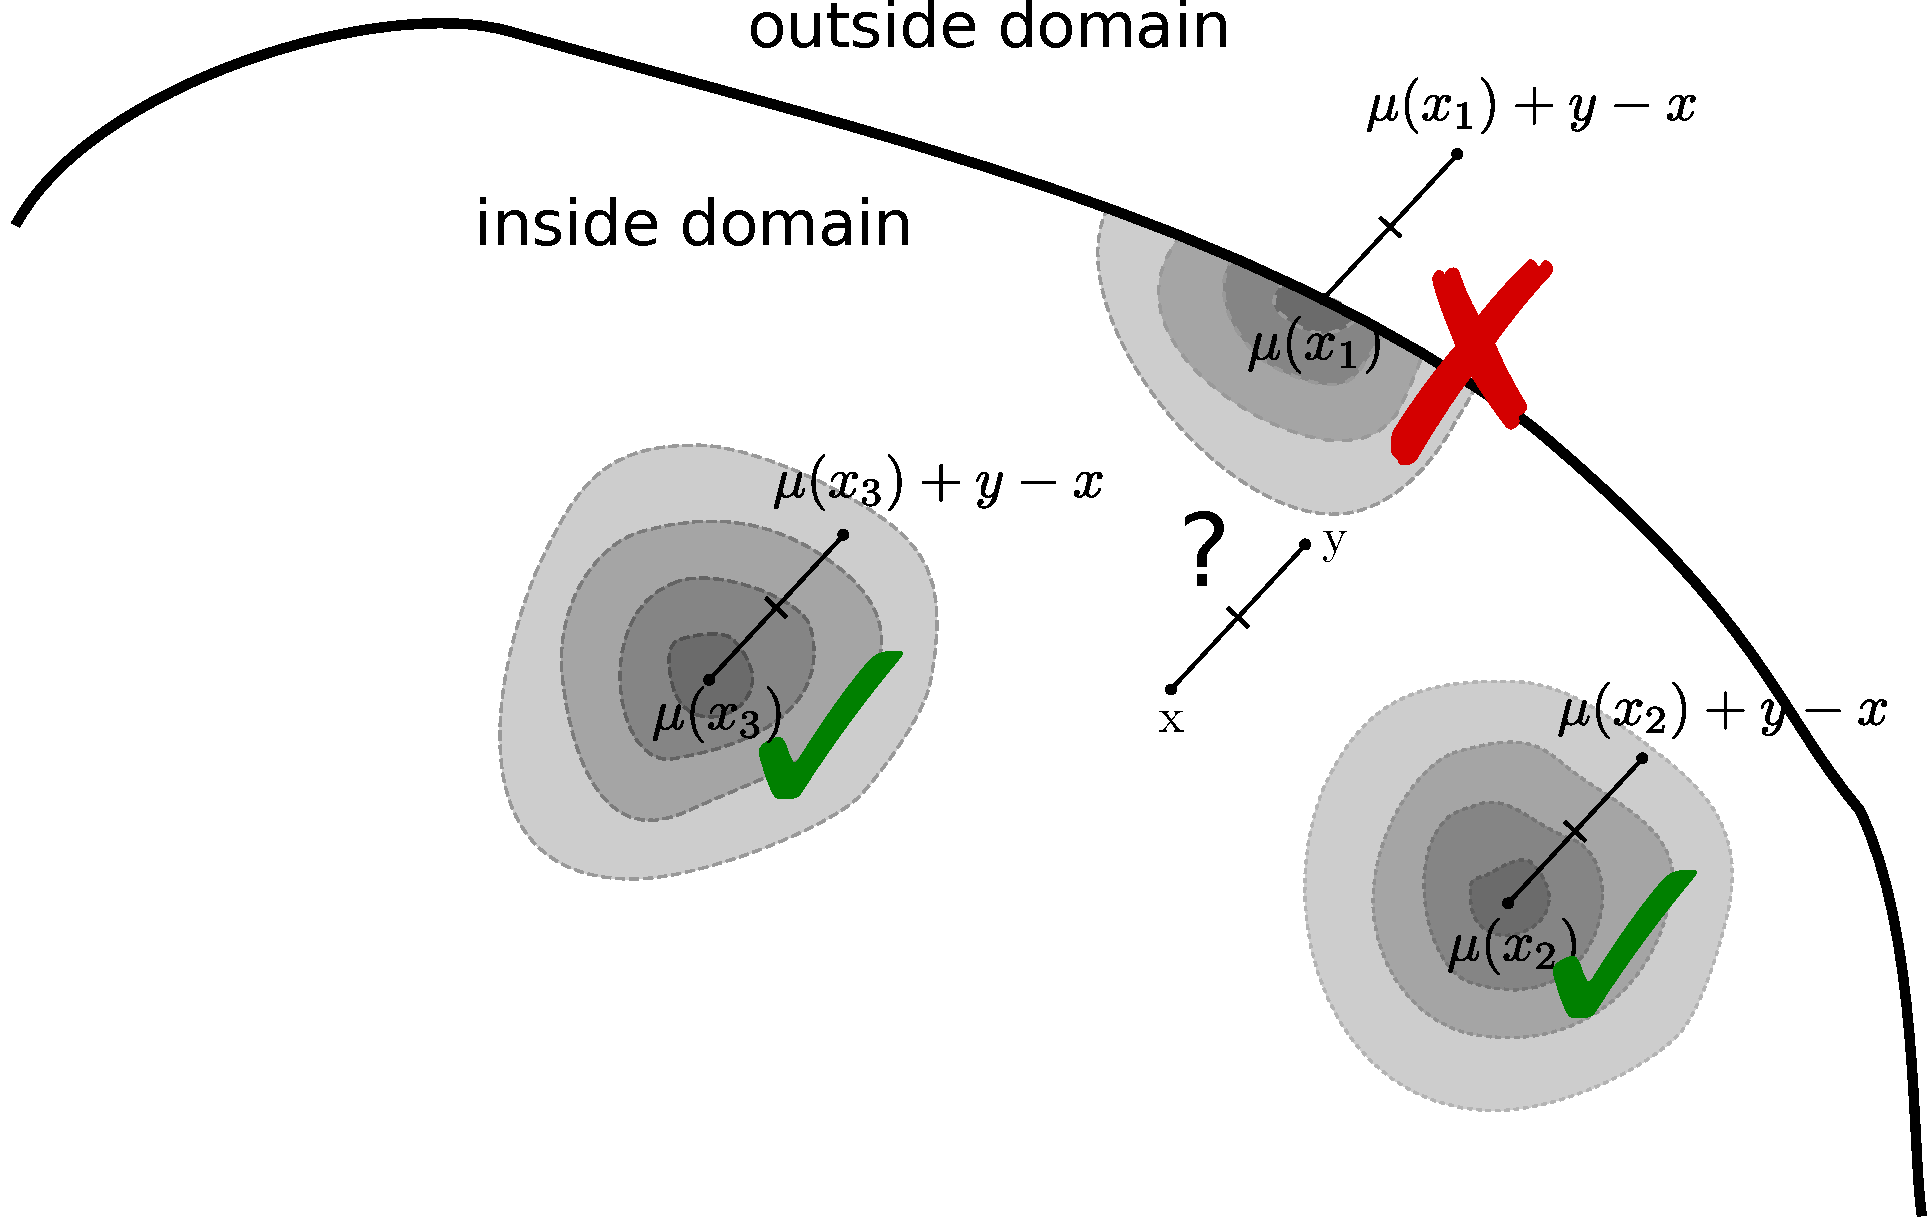
\includegraphics[scale=0.2]{interpolation_rbf_boundary.pdf}
	\caption{To compute the kernel entry $\Aker(y,x)$, we use radial basis functions to interpolate the values $\frac{\spatialvol(x)}{\spatialvol(x_i)}\phi_{x_i}(y-\spatialmean(x)-\spatialmean(x_i))$ for the $\numnbr$ nearest sample points $x_i$ to $x$, excluding sample points for which $y-\spatialmean(x)-\spatialmean(x_i)$ is outside of the domain.}
	\label{fig:rbf_interpolation}
\end{figure}

To evaluate $f_i$, we check whether $z_i \in E_{x_i}$ using \eqref{eq:support_ellipsoid}. If $z_i \notin E_{x_i}$, then $z_i$ is outside the estimated support of $\impulseresponse_{x_i}$, so we set $f_i=0$. If $z_i \in E_{x_i}$, we look up the batch index $b$ such that $x_i \in S_b$, and evaluate $f_i$ via the formula
\begin{equation}
f_i = \spatialvol(x)\eta_b\left(z_i\right),
\end{equation}
per \eqref{eq:varphi_eval}. 

 
Note that $z_i$ is generally not a gridpoint of the mesh used to discretize the problem, even if $y$, $x$, and $x_i$ are gridpoints. Hence,
evaluating $\eta_b\left(z_i\right)$ requires determining which mesh cell contains $z_i$, then evaluating finite element basis functions on that mesh cell. Fortunately, the mesh cell containing $z_i$ was already determined as a side effect of querying the AABB tree of mesh cells when we checked whether $z_i \in \Omega$. 



\subsection{Hierarchical matrix construction}
\label{sec:h_matrix_construction_short}

We form our H-matrix approximation $\mathbf{A}_H \approx \mathbf{A}$ by forming H-matrix representations $\mathbf{\Aker}_H$ and $\massmatrix_H$ of $\mathbf{\Aker}$ and $\massmatrix$, respectively, then using fast H-matrix methods to multiply these matrices per \eqref{eq:boldA} to form
\begin{equation*}
\mathbf{A}_H = \massmatrix_H \mathbf{\Aker}_H \massmatrix_H.
\end{equation*}
%Once $\mathbf{A}_H$ is formed, useful matrix operations such as matrix-vector products, matrix-matrix addition, matrix-matrix multiplication, and matrix inversion may be performed using fast scalable H-matrix methods \cite{BORMHACKBUSCHBOOK}. 
We use H1 matrices in our numerical results, but any of the other H-matrix formats (such as H2, HODLR, HSS, HBS, and others \cite{HMATRIX}) could be used instead. For more details on H-matrices, see \cite{Hackbusch15}. 

We form $\mathbf{\Aker}_H$ using the standard geometrical clustering/adaptive cross method implemented within the HLIBpro software package \cite{Kriemann08}. Although $\mathbf{\Aker}$ is a dense $\fedim \times \fedim$ matrix, constructing $\mathbf{\Aker}_H$ only requires evaluation of $O(\hrank^2 \fedim \log \fedim)$ entries $\mathbf{\Aker}_{ij} = \widetilde{\Aker}(p_i, p_j)$, and these entries are computed via the radial basis function interpolation method described in Section \ref{sec:approximate_kernel_entries}. Here $\hrank$ is the rank of the highest-rank block in the H-matrix. 
A dense representation of $\mathbf{\Aker}$ is never formed. 
%We describe this H-matrix construction process in detail in Appendix \ref{app:h_matrix}. 
We form $\massmatrix_H$ using standard H-matrix methods for sparse matrices implemented within HLIBpro, using the same recursive block partitioning structure as was used for $\mathbf{\Aker}$. 



\section{Computational cost}
\label{sec:overall_cost}

The computational cost of our method may be divided into the costs to perform the following tasks: (1) Computing impulse response moments and batches; (2) Building the H-matrix; (3) Performing linear algebra operations with the H-matrix. This may optionally include modifying the H-matrix to make it symmetric positive semi-definite.
In practice, (1) is the dominant cost, because (1) is the only task that requires applying $\Aop$ to vectors, and our method is targeted at applications in which applying $\Aop$ to a vector requires an expensive computational procedure such as solving a large-scale partial differential equation. All operations that do not require applications of $\Aop$ to vectors are nearly-linear, and therefore scalable, in the size of the problem, $N$.
We now describe these costs in detail. For convenience, Table \ref{tab:vars} lists variable symbols and their approximate sizes.

\begin{table}
	\begin{tabular}{lll}
		Symbol & Typical size & Variable name \\
		\hline
		$\fedim$ & $10^2$--$10^9$ & Number of finite element degrees of freedom \\
		$\nbatch$ & $1$--$25$ & Number of impulse response batches \\
		$\hrank$ & $5$--$50$ & H-matrix rank \\
		$\numnbr$ & $5$--$15$ & Number of nearest neighbors for RBF interpolation \\
		$\gdim$ & $1$--$3$ & Spatial dimension \\
%		$\classicalrank$ & $10^1$--$10^4$ & Classical matrix rank \\
		$\nsamplepts$ & $10^1$--$10^4$ & Total number of sample points (all batches) \\
		$|\pointbatch_i|$ & $1$--$500$ & Number of sample points in the $i$th batch \\
		$\ratord$ & $1$--$2$ & Rational function parameter for SPSD modification
	\end{tabular}
	\caption{Symbols used for variables in computational cost estimates, and approximate ranges for their sizes in practice.}
	\label{tab:vars}
\end{table}

\paragraph{(1) Computing impulse response moments and batches} Computing $\spatialvol$, $\spatialmean$, and $\spatialcov$ requires applying $\Aop$ to $1$, $\gdim$, and $\gdim(\gdim+1)/2$ vectors, respectively.
Computing each impulse response batch requires applying $\Aop$ to one vector, so computing the impulse response batches $\{\eta_i\}_{i=1}^{\nbatch}$ requires $\nbatch$ operator applies. In total, computing the impulse response moments and batches therefore requires
\begin{equation*}
	1 + \gdim + \gdim(\gdim+1)/2 + \nbatch \qquad \text{operator applies.}
\end{equation*}
In a typical application one might have $\gdim=2$ and $\nbatch=5$, in which case a modest $11$ operator applies are required.

Computing the impulse response batches also requires choosing sample point batches via the greedy ellipsoid packing algorithm described in Section \ref{sec:sample_point_selection}. Choosing the $i$th batch of sample points may require performing up to $\fedim |\pointbatch_i|$ ellipsoid intersection tests, where $|\pointbatch_i|$ is the number of sample points in the $i$th batch. Choosing all of the sample points therefore requires performing at most
\begin{equation*}
	\fedim \nsamplepts \qquad \text{ellipsoid intersection tests,}
\end{equation*}
where $\nsamplepts$ is the total number of sample points in all batches. The multiplicative dependence of $\fedim$ with $\nsamplepts$ is undesirable since $\nsamplepts$ may be large, and reducing this cost is a target for future work. 
%Several improvements are possible. The cost of picking sample points could be reduced by ``thinning'' the set of candidate points that the sample points are picked from. That is, choosing sample points from a smaller subset of $\fedim_\text{thin} << \fedim$ points. The cost to perform the ellipsoid intersection tests could be reduced by first checking whether the ellipsoid bounding boxes intersect before performing the ellipsoid intersection test of Appendix \ref{sec:fast_ellipsoid_intersection_test}. The cost of picking the $i$th batch could be reduced to $O(\fedim \log |\pointbatch_i|)$ using more advanced computational geometry techniques, such as organizing the ellipsoids associated with points that have already been picked into a dynamic AABB tree, then using this AABB tree to accelerate the required ellipsoid intersection tests. 
However, from a practical perspective, the cost for picking sample points is small compared to other parts of the approximation algorithm, so we do not pursue these improvements in this paper.

\paragraph{(2) Building the H-matrix} The classical H-matrix construction technique
%, which is described in Appendix \ref{app:h_matrix}, 
requires evaluating $O(\hrank^2 \fedim \log \fedim)$ matrix entries of the approximation, where $\hrank$ is the H-matrix rank, i.e,  the maximum rank among the blocks of the H-matrix. To evaluate one matrix entry, first one must find the $\numnbr$ nearest sample points to a given point, where $\numnbr$ is the number of impulses used in the RBF interpolation. This is done using a precomputed KD tree of sample points, and requires $O(\numnbr \log \nsamplepts)$ floating point and logical elementary operations. Second, one must find the mesh cells that the points $\{z_i\}_{i=1}^{\numnbr}$ reside. This is done using an AABB tree of mesh cells, and requires $O(\numnbr \log \fedim)$ elementary operations. Third, we must evaluate finite element basis functions on each of those cells, which requires $O(\numnbr)$ elementary operations. Finally, we must solve a $\numnbr \times \numnbr$ linear system to perform the radial basis function interpolation, which requires $O(\numnbr^3)$ elementary operations, which typically is negligible. Therefore, building the H-matrix requires
\begin{equation*}
	O\left(\left(\hrank^2 \fedim \log \fedim\right)\left(\numnbr \log \fedim + \numnbr^3\right)\right) \qquad \text{elementary operations}.
\end{equation*}
%This follows from the above discussion, and the fact that $\fedim \ge \nsamplepts$.

\paragraph{(3) Performing linear algebra operations with the H-matrix} It is well-known that H-matrix methods for matrix-vector products, matrix-matrix addition, matrix-matrix multiplication, matrix factorization, and matrix inversion, and low rank updates require
\begin{equation}
\label{eq:H_matrix_cost_operations}
	O(\hrank^2 \fedim \log(\fedim)^a) \qquad \text{elementary operations},
\end{equation}
where $a \in \{0,1,2,3\}$ \cite{GrasedyckHackbusch03}. The precise cost depends on the type of H-matrix used and the operation being performed. In this paper, we use one matrix-matrix addition to add the H-matrix approximation of the data misfit term in the Hessian to the regularization term in the Hessian. Then, we use one matrix inversion to form the inverse of the Hessian, which is used as a preconditioner for the Newton linear system. 
%We perform low-rank updates to the H-matrix as the Newton iterations proceed, as per the discussion in Appendix \ref{sec:recycle_krylov}.
The rational method for modifying $\mathbf{A}_H$ to be positive semi-definite, described in Appendix \ref{sec:make_spd}, is performed using two matrix-matrix additions, $\ratord+1$ matrix-matrix multiplications, and one matrix inversion, where $2^\ratord$ is the order of the rational function used.


\section{Numerical results}
\label{sec:numerical_results}

%\textbf{Heat equation}
%\begin{itemize}
%	\item Hessian per-column error plots for 1, 5, and 15 batches
%	\item $H-P$ error vs number of batches for interior and whole domain
%	\item $P^{-1}H-I$: error vs rank for $P=R$ and $P=P_\text{pch}$ diffusion time, for 1, 5, and 15 batches
%	\item Krylov iterations to tols 1e-1 and 1e-6 vs diffusion parameter
%	\item GLR vs PCH vs diffusion time
%	\item Krylov method convergence plot: $R$ vs $P_\text{pch}$ vs no preconditioner
%	\item Krylov iterations to tols 1e-6 vs mesh size $h$, PCH vs R vs no preconditioner (hold)
%	\item true parameter (H)
%	\item deterministic reconstruction (H)
%	\item noisy measurements (1\%, 5\%, 10\% noise). $u|_\text{top}$ (H)
%	\item recovered state at top (H)
%	\item mesh scalability of PCH (CC) (H)
%	\item put plot data into data directory
%	\item save function .pvd files in paraview  directory
%\end{itemize}
%
%\begin{itemize}
%	\item GLR vs PCH number of obs (Computational cost in PDE solves) (S)
%	\item GLR vs PCH aspect ratio (CC) (S)
%	\item turn on preconditioner after number of krylov iterations exceeds 15 in an iteration. Rebuild "as needed". (S)
%\end{itemize}
%
%\begin{itemize}
%	\item Stokes Krylov convergence (10 solves for nonlinear forward + 6 hessian matvecs for ellipsoid estimation + 10 matvecs for impulse responses + 30 matvecs for PCH6 CG solve + 100 matvecs for Reg CG solve)
%	\item Stokes error vs num batches (small number of batches; 1, 3, 6, 9 batches?) (50 matvecs for randomized error estimation +)
%	\item Velocity field
%	\item Basal friction field
%	\item Picture of impulse responses
%	\item Mesh negative numbers picture
%\end{itemize}
%
%\begin{itemize}
%	\item mtrue
%	\item utrue (no arrows)
%	\item utrue (yes arrows)
%	\item reconstruction iterations 1,3,4,8: PCH vs REG
%	\item urecovered (arrows, 3D)
%	\item morozov plot
%	\item Newton convergence (iter, numcg, numPDEsolves (num preconditioner build), gradnorm)
%	\item impulse response batches
%	\item 
%\end{itemize}

Some numerical results here.

\begin{figure}[H]
	\begin{center}
		\begin{tabular}[c]{c c c}
			%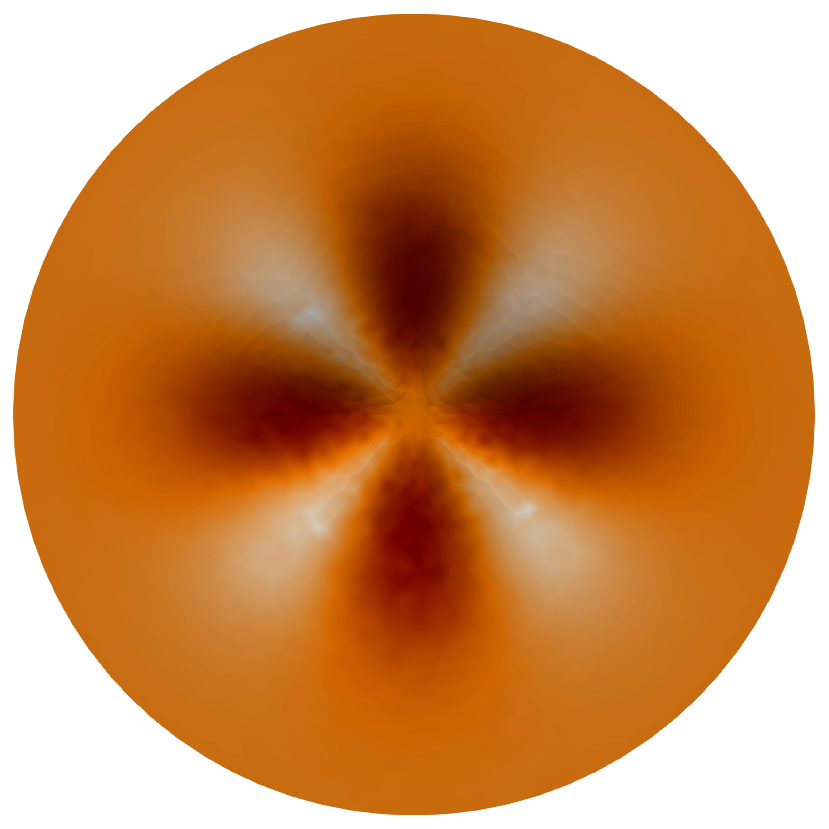
\includegraphics[scale=.15]{recoveredPressure.png} &
			%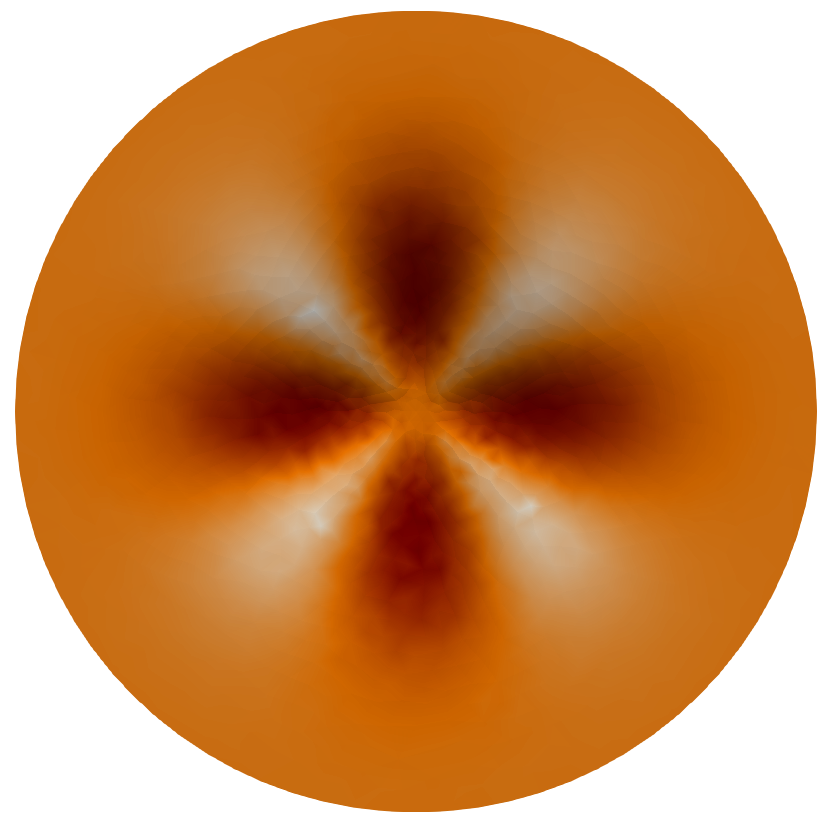
\includegraphics[scale=.15]{truePressure.png} &
			%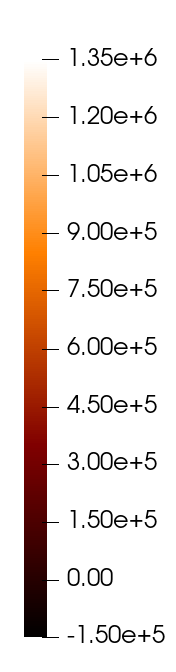
\includegraphics[scale=.18]{pressureColorBar.png} \\
			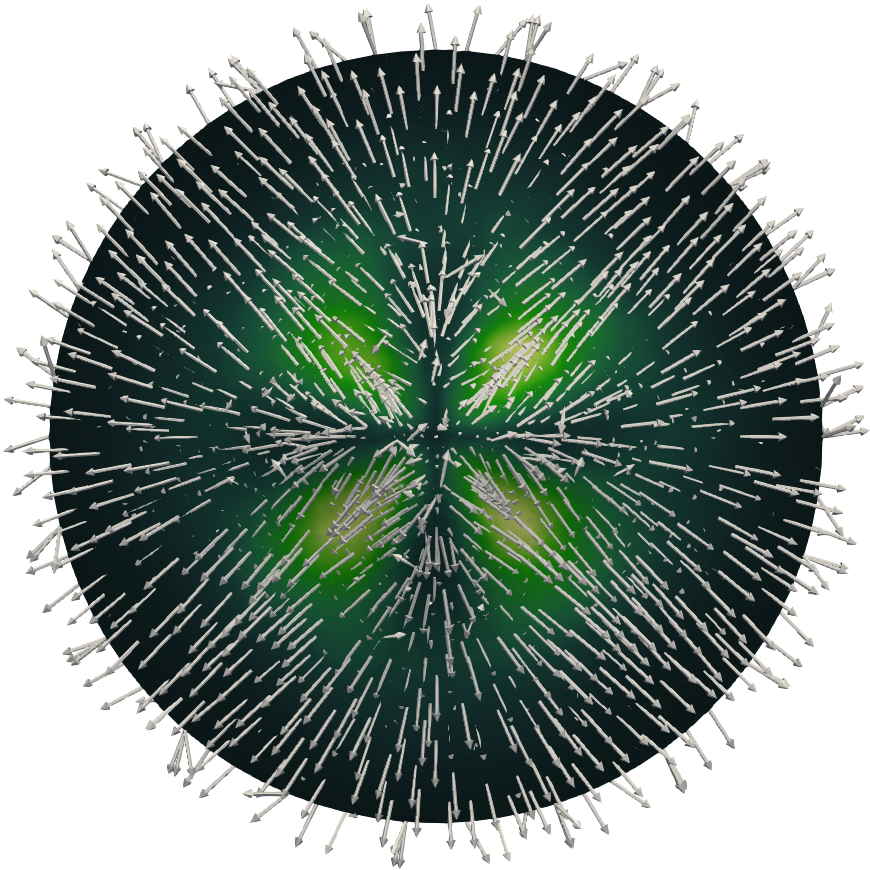
\includegraphics[scale=.15]{recoveredVelocity_glyphs.png} &
			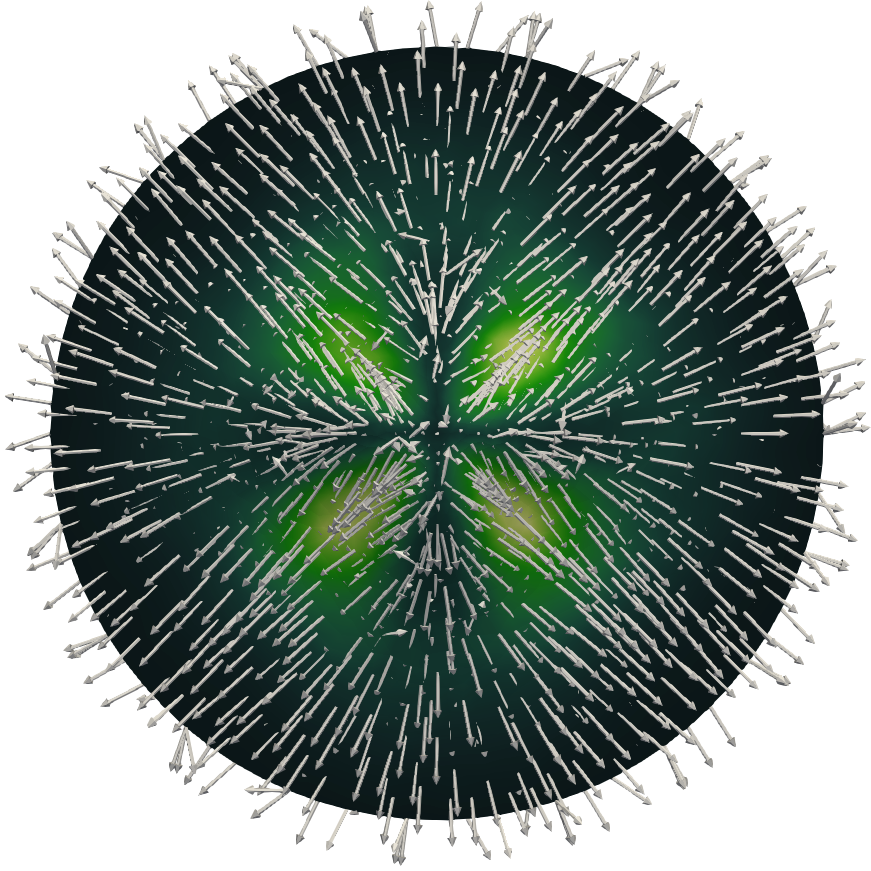
\includegraphics[scale=.15]{trueVelocity_glyphs.png} &
			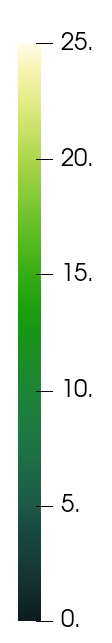
\includegraphics[scale=.18]{velocityColorBar.png} \\
			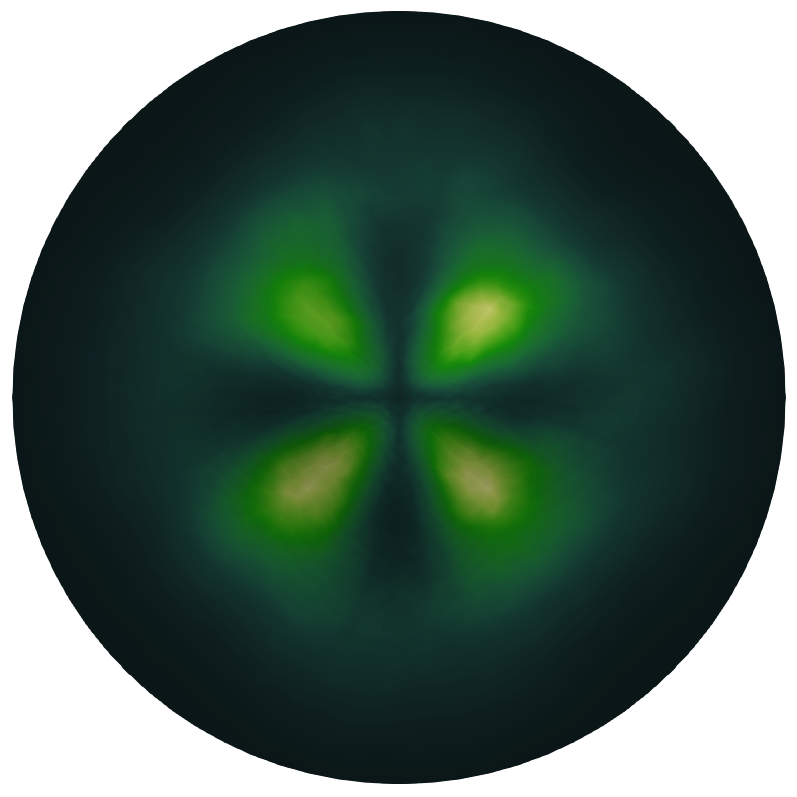
\includegraphics[scale=.15]{recoveredVelocity_noglyphs.png} &
			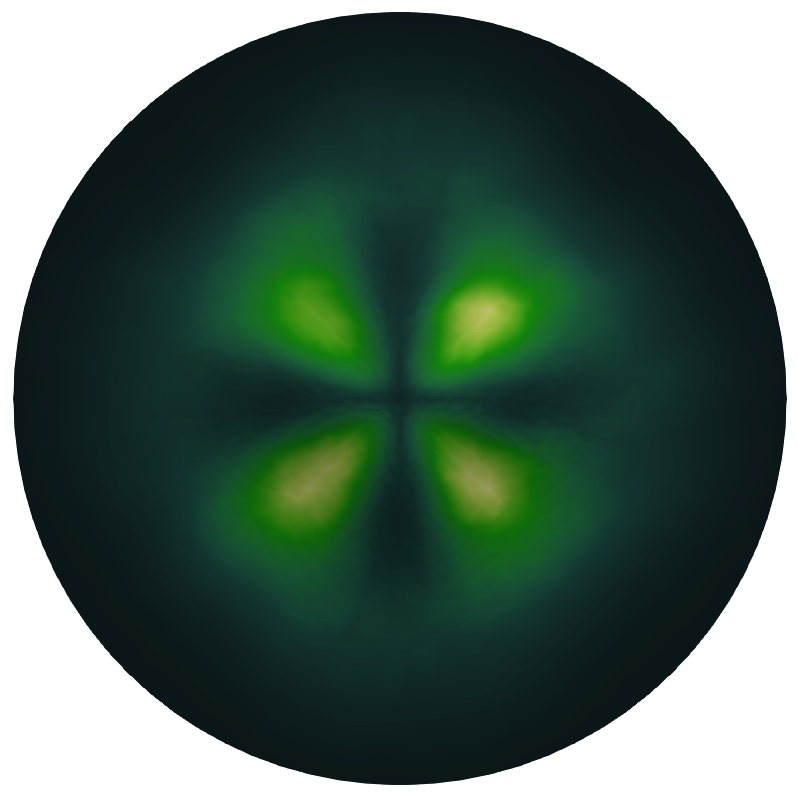
\includegraphics[scale=.15]{trueVelocity_noglyphs.png} &
			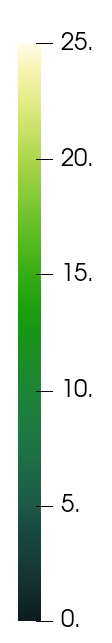
\includegraphics[scale=.18]{velocityColorBar.png}
		\end{tabular}
		\caption{Reconstructed (left column) and true (right column) pressure (top row) and velocity fields (middle and bottom rows).}
	\end{center}
\end{figure}


\begin{table}[H]
	\begin{center}
		\begingroup
		\setlength{\tabcolsep}{4pt}
		\renewcommand{\arraystretch}{1.25}
		\begin{tabular}{c| c c c | c c c | c c c}
			&  \multicolumn{3}{|c|}{PSF} & \multicolumn{3}{|c|}{REG} & \multicolumn{3}{|c}{NONE} \\
			\hline
			Iter & 
			\#CG & \#Stokes & $||g||$ & 
			\#CG & \#Stokes & $||g||$ & 
			\#CG & \#Stokes & $||g||$ \\
			\verb~0~ &
			\verb~1~ & \verb~4~ & \verb~1.95e+7~ &
			\verb~1~ & \verb~4~ & \verb~1.95e+7~ &
			\verb~1~ & \verb~4~ & \verb~1.95e+7~ \\
			\verb~1~ &
			\verb~2~ & \verb~6~ & \verb~5.76e+6~ &
			\verb~2~ & \verb~6~ & \verb~7.90e+6~ &
			\verb~2~ & \verb~6~ & \verb~5.76e+6~ \\
			\verb~2~ &
			\verb~4~ & \verb~10~ & \verb~2.36e+6~ &
			\verb~5~ & \verb~12~ & \verb~3.87e+6~ &
			\verb~4~ & \verb~10~ & \verb~2.36e+6~ \\
			\verb~3~ &
			\verb~2~ & \verb~6+22~ & \verb~5.79e+5~ &
			\verb~13~ & \verb~28~ & \verb~1.62e+6~ &
			\verb~13~ & \verb~28~ & \verb~5.79e+5~ \\
			\verb~4~ &
			\verb~5~ & \verb~12~ & \verb~5.61e+4~ &
			\verb~42~ & \verb~86~ & \verb~4.78e+5~ &
			\verb~33~ & \verb~68~ & \verb~9.05e+4~ \\
			\verb~5~ &
			\verb~10~ & \verb~22~ & \verb~3.45e+3~ &
			\verb~84~ & \verb~170~ & \verb~7.72e+4~ &
			\verb~57~ & \verb~116~ & \verb~6.21e+3~ \\
			\verb~6~ &
			\verb~14~ & \verb~30~ & \verb~2.66e+1~ &
			\verb~125~ & \verb~252~ & \verb~5.04e+3~ &
			\verb~76~ & \verb~154~ & \verb~1.05e+2~ \\
			\verb~7~ &
			\verb~0~ & \verb~2~ & \verb~4.09e-2~ &
			\verb~194~ & \verb~390~ & \verb~7.91e+1~ &
			\verb~117~ & \verb~236~ & \verb~2.29e-1~ \\
			\verb~8~ & 
			\verb~---~ & \verb~---~ & \verb~---~ &
			\verb~0~ & \verb~2~ & \verb~1.60e-1~ &
			\verb~0~ & \verb~2~ & \verb~4.08e-2~ \\
			\hline
			Total & 
			\verb~38~ & \verb~114~ & \verb~---~ &
			\verb~466~ & \verb~950~ & \verb~---~ &
			\verb~303~ & \verb~624~ & \verb~---~ \\
		\end{tabular}
		\endgroup
	\end{center}
\end{table}





             




\begin{figure}[H]
\begin{subfigure}{0.49\textwidth}
	\centering
	\begin{tikzpicture}[baseline, trim axis right]
	\begin{axis}[width=0.99\linewidth, height=1.0\linewidth,
	ymode=log,
	ymin=1e-11,
	ymax=2,
	xmax=750,
	axis x line*=bottom,
	axis y line*=left,
	xtick={0, 200, 400, 600},
	xlabel={CG iteration},
	ylabel={Relative residual norm},
	title={CG convergence},
	legend style={at={(1.1,1)},anchor=north east},
	%legend pos=north east,
	legend style={font=\small}
	]
	\addlegendentry{PSF (1)}
    \addplot[blue, line width=0.5mm] table {cg_relres_p1.dat};
    \addlegendentry{PSF (5)}
    \addplot[red, line width=0.5mm] table {cg_relres_p5.dat};
    \addlegendentry{PSF (25)}
    \addplot[purple, line width=0.5mm] table {cg_relres_p25.dat};
	\addlegendentry{Reg}
    \addplot[dotted, line width=0.5mm] table {cg_relres_reg.dat};
	\addlegendentry{None}
	\addplot[dash dot, line width=0.5mm] table {cg_relres_none.dat};
	\end{axis}
	\end{tikzpicture}
\end{subfigure}
	\begin{subfigure}{0.49\textwidth}
		\centering
		\begin{tikzpicture}[baseline, trim axis right]
		\begin{axis}[width=0.99\linewidth, height=1.0\linewidth,
		xmode=log,
		ymode=log,
		xlabel={$\gamma$, regularization parameter},
		ylabel={\# of CG iterations},
		axis y line*=right,
		axis x line*=bottom,
		ylabel near ticks, yticklabel pos=right,
		%ylabel near ticks, ylabel shift={-6pt},
		%legend pos=north east,
		title={Regularization robustness}
		%title={CG iterations to achieve $||H x-b||/||b||<10^{-6}$}
		]
		%\addlegendentry{None}
		\addplot[dash dot, line width=0.5mm] table[x=gamma, y=none] {CGitsvsGamma.dat};
		%\addlegendentry{REG}
		\addplot[dotted, line width=0.5mm] table[x=gamma, y=reg] {CGitsvsGamma.dat};
		%\addlegendentry{PSF (1)}
        \addplot[blue, line width=0.5mm] table[x=gamma, y=psf1] {CGitsvsGamma.dat};
        %\addlegendentry{PSF (5)}
        \addplot[red, line width=0.5mm] table[x=gamma, y=psf5] {CGitsvsGamma.dat};
        %\addlegendentry{PSF (25)}
        \addplot[purple, line width=0.5mm] table[x=gamma, y=psf25] {CGitsvsGamma.dat};
		\end{axis}
		\end{tikzpicture}
	\end{subfigure}
\end{figure} 

\begin{figure}[H]
	\begin{subfigure}{0.59\textwidth}
	\begin{center}
		\begin{tikzpicture}[baseline, trim axis right]
		\begin{axis}[width=0.99\linewidth, height=0.8\linewidth,
		ymode=log,
		xmin=-50,
		xmax=1450,
		ymax=1.e4,
		xlabel={$k$, generalized eigenvalue \#},
		ylabel={$\lambda_{k}$},
		xtick={0, 300, 600, 900, 1200},
		%legend pos=north east,
		legend style={font=\small},
		ylabel near ticks, ylabel shift={-6pt},
		axis x line*=bottom,
		axis y line*=left,
		legend style={at={(0.95,1)},anchor=north east},
		title={Generalized eigenvalues, $Hu_{k}=\lambda_{k}Pu_{k}$}
		]
		\addlegendentry{PSF (1)}
        \addplot[blue, line width=0.5mm] table[x=k, y=psf1] {generalizedEigenvalues.dat};
        \addlegendentry{PSF (5)}
        \addplot[red, line width=0.5mm] table[x=k, y=psf5] {generalizedEigenvalues.dat};
        \addlegendentry{PSF (25)}
        \addplot[purple, line width=0.5mm] table[x=k, y=psf25] {generalizedEigenvalues.dat};
		\addlegendentry{REG}
		\addplot[dotted, line width=0.5mm] table[x=k, y=reg] {generalizedEigenvalues.dat};
		\end{axis}
		\end{tikzpicture}
	\end{center}
\end{subfigure}
\begin{subfigure}{0.39\textwidth}
		\begin{center}
		\begingroup
		\setlength{\tabcolsep}{4pt}
		\renewcommand{\arraystretch}{1.25}
		\begin{tabular}{c| c c}
			& $\kappa(P^{-1}H)$ &	$\kappa(P^{-1}H_{\text{gn}})$ \\
			\hline 
			PSF $(1)$  & \verb~1.8e+1~ & \verb~1.8e+1~ \\
            PSF $(5)$  & \verb~1.4e+1~ & \verb~1.4e+1~ \\
            PSF $(25)$ & \verb~1.0e+1~ & \verb~1.1e+1~ \\
			REG        & \verb~7.0e+3~ & \verb~7.0e+3~ \\
			NONE       & \verb~8.7e+2~ & \verb~9.2e+2~ 
		\end{tabular}
		\endgroup
	\end{center}
\end{subfigure}
\end{figure}


\section{Conclusions}
\label{sec:conclusions}

Some conclusions here. 

Although the method we present in this paper is not applicable to all Hessians, it is applicable to several Hessians of practical interest. For these Hessians, our method offers a \emph{data-scalable} alternative to conventional low-rank Hessian approximation methods, because our method can form high rank approximations of an operator using a small number of matrix-vector products.

\appendix


%\section{Hierarchical matrix details}
%\label{app:h_matrix}
%
%Often, large dense matrices of practical interest may be permuted, then partitioned into blocks recursively, in such a way that many off-diagonal blocks of the matrix are numerically low rank, even if the matrix is high rank. Such matrices are known as hierarchical matrices (H-matrices). Many classes of H-matrices exist (H1, H2, HSS, HBS, and more), and all of these types of H-matrices could be used in conjunction with our product-convolution approximation. Here we use classical H1 matrices. For this section, when we say H-matrix, we are referring to H1 matrices. 
%
%While a dense $\fedim \times \fedim$ matrix traditionally requires $O(\fedim^2)$ memory to store, H-matrices may be stored using $O(\fedim \log \fedim)$ memory, by storing only the low rank factors for the low rank blocks. Recursive algorithms can take advantage of the H-matrix low rank block structure to perform matrix arithmetic fast. Conventional dense matrix algorithms for matrix inversion, matrix factorization, matrix-vector products, matrix-matrix products, and matrix-matrix addition require either $O(\fedim^2)$ or $O(\fedim^3)$ time and memory, while the aforementioned recursive algorithms can perform these matrix operations in $O(\fedim \log(\fedim)^a)$ time and memory for H-matrices. Here $a=0, 1, 2$, or $3$ depending on the operation and type of H-matrix. For more details on H-matrices, we recommend \cite{HMATRIXGOOD}. 
%
%
%\subsection{H-matrix construction}
%\label{sec:H_matrix_construction}
%
%The process of constructing an H-matrix representation of $\mathbf{\Aker}$ proceeds as follows. First, we construct hierarchical partitionings of the degrees of freedom for the columns and rows of the matrix (cluster trees, Section \ref{sec:cluster_trees}). Second, we construct a hierarchical partitioning of the blocks of the matrix, in such a way that many of the blocks in the partitioning are expected to be low rank, and the remaining high rank blocks are small (block cluster tree, Section \ref{sec:block_cluster_tree}). Finally, we form low rank approximations of the blocks of the matrix that are expected to be low rank (adaptive cross approximation, Section \ref{sec:adaptive_cross}), and fill in the remaining high rank  blocks with their numerical values. The first two steps require geometric information about the spatial locations of the degrees of freedom associated with the rows and columns of the matrix, but these steps do not depend on the particular values of matrix entries. The third step requires us to evaluate $O(\fedim \log \fedim)$ specially-chosen entries of $\mathbf{\Aker}$, and we evaluate these entries using \eqref{eq:Akerpcmat_entries}. 
%
%
%\subsubsection{Cluster trees}
%\label{sec:cluster_trees}
%
%We use recursive hyperplane splitting to hierarchically cluster the degrees of freedom associated with the columns and rows of the matrix into a \emph{column cluster tree} and a \emph{row cluster tree}, respectively. Here we describe construction of the column cluster tree; the row cluster tree is constructed similarly. 
%
%Since we use finite elements to discretize the problem, the $i^\text{th}$ column of $\mathbf{\Aker}$ corresponds to the Lagrange node in $\mathbb{R}^\gdim$ associated with the $i\text{th}$ finite element basis function. The columns of the matrix thus correspond to a point cloud in $\mathbb{R}^\gdim$. We split this point cloud into two equally sized \emph{child} point clouds, using a hyperplane which is perpendicular to the coordinate axis direction in which the point cloud is widest (e.g., either the $x$, $y$, or $z$ axis in $3$D). The two child point clouds are split in the same way. This splitting process repeats until the point clouds have less than a preset number of points (we use $32$ points). This hierarchical partitioning of the point cloud into smaller and smaller point clouds corresponds to a hierarchical partitioning of the columns of the matrix into smaller and smaller \emph{clusters} of columns. This hierarchical partitioning of the columns forms a binary tree, which is called the column cluster tree. The root of the tree is the set of all columns, and the leaves of the tree are clusters of columns that are not subdivided any further. 
%
%A depth-first search ordering of the column cluster tree leaves is then generated. When the columns of the matrix are permuted into this depth-first ordering, the columns associated with each cluster in the cluster tree are contiguous.
%
%In the same way, the degrees of freedom associated with the rows of the matrix are hierarchically clustered into another cluster tree, and a depth-first search ordering for the rows is generated. In our examples, the degrees of freedom for the columns coincide with the degrees of freedom for the rows, so the cluster trees for the rows and columns are the same, but this is not required in general.
%
%
%\subsubsection{Block cluster tree} 
%\label{sec:block_cluster_tree}
%
%We partition the matrix into a recursive hierarchy of mostly low rank blocks called the \emph{block cluster tree}. The idea is that a block of the matrix is likely to be low rank if the point cloud associated with the rows of the block is far away from the point cloud associated with the columns of the block. This is reasonable to expect here because of the locality property of $\Aop$. Indeed, locality implies that many blocks of the matrix corresponding to far away point cloud clusters will be rank zero.
%
%After reordering the rows and columns of $\mathbf{\Aker}$ via the depth-first ordering described above, we partition the reordered version of $\mathbf{\Aker}$ into a tree of $2 \times 2$ block matrices recursively. We use a geometric admissibility condition (discussed below) to decide which blocks to subdivide, and use the cluster trees for the rows and columns to determine how to subdivide those blocks. For the first stage of subdivision, let $r_1$ and $r_2$ be the children row clusters for the root of the row cluster tree, let $\colcluster_1$ and $\colcluster_2$ be the children column clusters for the root of the column cluster tree. The matrix $\mathbf{\Aker}$ is partitioned into blocks as follows:
%\begin{equation*}
%	\begin{bmatrix}
%		\mathbf{\Aker}_{11} & \mathbf{\Aker}_{12} \\
%		\mathbf{\Aker}_{21} & \mathbf{\Aker}_{22}
%	\end{bmatrix},
%\end{equation*}
%where $\mathbf{\Aker}_{11}$ denotes the block of $\mathbf{\Aker}$ with rows $r_1$ and columns $\colcluster_1$, $\mathbf{\Aker}_{12}$ denotes the block of $\mathbf{\Aker}$ with rows $r_1$ and columns $\colcluster_2$, and so on for $\mathbf{\Aker}_{21}$ and $\mathbf{\Aker}_{22}$.
%
%We now loop through the four blocks, $\mathbf{\Aker}_{11}$, $\mathbf{\Aker}_{12}$, $\mathbf{\Aker}_{21}$, and $\mathbf{\Aker}_{22}$, and decide which blocks should be subdivided further. For the purpose of explanation, consider $\mathbf{\Aker}_{12}$. If
%\begin{equation}
%	\label{eq:weak_admissibility_cond}
%	\dist\left(r_1, \colcluster_2\right) \ge \weakadmconst \min\left(\diam\left(r_1\right), \diam\left(\colcluster_2\right)\right),
%\end{equation}
%then we mark $\mathbf{\Aker}_{12}$ as \emph{admissible} (expected to be low rank) and leave it alone. Here $\dist\left(r_1, \colcluster_2\right)$ is the Euclidean distance between the axis-aligned bounding box for the point cloud associated with the row cluster $r_1$, and the axis aligned bounding box for the point cloud associated with the column cluster $\colcluster_2$. The quantity $\diam\left(r_1\right)$ is the diameter of the axis aligned bounding box for the point cloud associated with the row cluster $r_1$, and $\diam\left(\colcluster_2\right)$ is the analogous diameter associated with the column cluster $\colcluster_2$. Here the quantity $\weakadmconst$ is a scalar constant; we use $\weakadmconst=2.0$. Basically, if the point clouds associated with $r_1$ and $\colcluster_2$ are far away from each other relative to their diameters, then we expect that the corresponding block of the matrix will be low rank. This process is repeated for the other blocks to determine which blocks are admissible and which are not. For us, the diagonal blocks $\mathbf{\Aker}_{11}$ and $\mathbf{\Aker}_{22}$ are not admissible because the distance between a point cloud and itself is zero. 
%
%Next, we subdivide all blocks that are not admissible and are larger than a predetermined size (we use size $32 \times 32$), using the same process that was used to subdivide $\mathbf{\Aker}$. But now we subdivide a block based on the two child row clusters and two child column clusters for the rows and columns of that block. This subdivision process continues recursively until all blocks are either admissible, or smaller than the predetermined size mentioned above. The resulting hierarchical partitioning of matrix blocks forms a tree, which is called the \emph{block cluster tree}. The root of the tree is the whole matrix, internal nodes in the tree are blocks that are subdivided, and the leaves of the tree are blocks that are either expected to be low rank, or are small.
%
%
%\subsubsection{Adaptive cross low rank approximation of blocks}
%\label{sec:adaptive_cross}
%
%Once the block cluster tree has been constructed, low rank approximations of the admissible (low rank) blocks are formed using the adaptive cross method \cite{ACA}. Let $X \in \mathbb{R}^{m \times m}$ be an admissible block of $\mathbf{\Aker}$. The idea of the adaptive cross method is to form a low rank approximation of $X$ by sampling a small number of rows and columns of $X$. 
%\begin{itemize}
%	\item Let $C \in \mathbb{R}^{m \times \hrank}$ be a matrix consisting of a subset of $\hrank$ columns of $X$, such that the span of the columns in $C$ approximates the column space of $X$. 
%	\item Let $R\in\mathbb{R}^{\hrank \times m}$ be a subset of the rows of $X$, such that the span of the rows in $R$ approximates the row space of $X$.
%	\item Let $U \in \mathbb{R}^{\hrank \times \hrank}$ be the block of $X$ consisting of the intersection of the rows from $R$ with the columns from $C$.
%\end{itemize}
%Then it is well-established that
%\begin{equation}
%	\label{eq:CUR}
%	X \approx C U^+ R,
%\end{equation}
%where $U^+$ is the pseudoinverse of $U$ \cite{goreinov1997theory,MahoneyDrineas09}. The quality of approximation \eqref{eq:CUR} depends on how well the columns of $C$ approximate the column space of $X$, and how well the rows of $R$ approximate the row space of $X$. 
%
%In the adaptive cross method, ``good'' columns, $C$, and rows, $R$, are chosen via an alternating iterative process. An initial set of columns $C$ is chosen. Keeping $C$ fixed, a set of rows $R$ is chosen so that the so that determinant of the submatrix $U$ within $C$ is as large as possible \cite{GoreinovEtAl10}. Now, keeping $R$ fixed, a set of new columns $C$ is chosen so that the submatrix $U$ within $R$ is as large as possible. This process repeats a small number of times. This results in matrices $R$ and $C$ such that the error in the approximation, \eqref{eq:CUR}, is small. The dominant cost of this procedure is the cost of computing $a \hrank$ columns of $X$ and $a\hrank$ rows of $X$, where $a$ is the number of alternating iterations. There is also a small linear algebra overhead cost for the determinant maximization process that is performed at each step. 
%The key point is that the adaptive cross method allows us to form a rank-$\hrank$ approximation of an $m \times m$ block of the matrix via a process that only requires accessing $O(m\hrank)$ entries of that block.
%
%We use the adaptive cross method to form low rank approximations for each admissible block of $\mathbf{\Aker}$. We directly compute all entries of the small dense blocks of $\mathbf{\Aker}$ that are not admissible. This process requires us to compute $O(\hrank^2 \fedim \log \fedim)$ entries of $\mathbf{\Aker}$, which is relatively cheap compared to the operator actions of $\Aop$ that are required to form the product-convolution approximation.


\section{Ellipsoid intersection test}
\label{sec:fast_ellipsoid_intersection_test}
The procedure for choosing sample points relies on quickly determining whether two ellipsoids intersect. Let $E_1$ and $E_2$ be the ellipsoids defined as
\begin{align*}
	E_1 :=& \{x : (x - \spatialmean_1)^T \spatialcov_1^{-1} (x - \spatialmean_1) \le \tau^2\}, \\
	E_2 :=& \{x : (x - \spatialmean_2)^T \spatialcov_2^{-1} (x - \spatialmean_2) \le \tau^2\}, \\
\end{align*}
where $\spatialmean_1, \spatialmean_2 \in \mathbb{R}^\gdim$, and $\spatialcov_1, \spatialcov_2 \in \mathbb{R}^{\gdim \times \gdim}$ are positive definite. Let $K$ be the following one dimensional convex function:
\begin{equation*}
	K(s) := 1 - \frac{1}{\tau^2} (\spatialmean_1 - \spatialmean_2)^T \left(\frac{1}{1-s}\spatialcov_1 + \frac{1}{s}\spatialcov_2\right)^{-1}(\spatialmean_1 - \spatialmean_2)	
\end{equation*}
In \cite{GilitschenskiHanebeck12} it is shown that $E_1 \cap E_2 = \{\}$ if and only if $K(s) < 0$ for some $s\in (0,1)$. We check whether $E_1$ and $E_2$ intersect by minimizing $K(s)$ on $(0,1)$. If $K(s^*) <0$ at the minimizer $s^*$, then $E_1 \cap E_2 = \{\}$. Otherwise $E_1 \cap E_2 \neq \{\}$.

\begin{figure}
	\begin{subfigure}{0.32\textwidth}
		\centering
		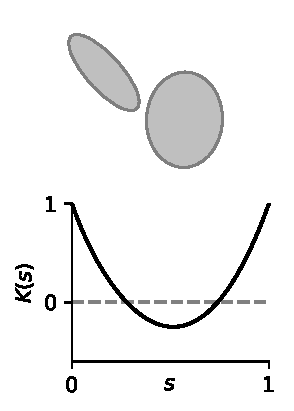
\includegraphics[scale=0.40]{ellipsoids_intersect0.pdf}
	\end{subfigure}
	\begin{subfigure}{0.32\textwidth}
		\centering
		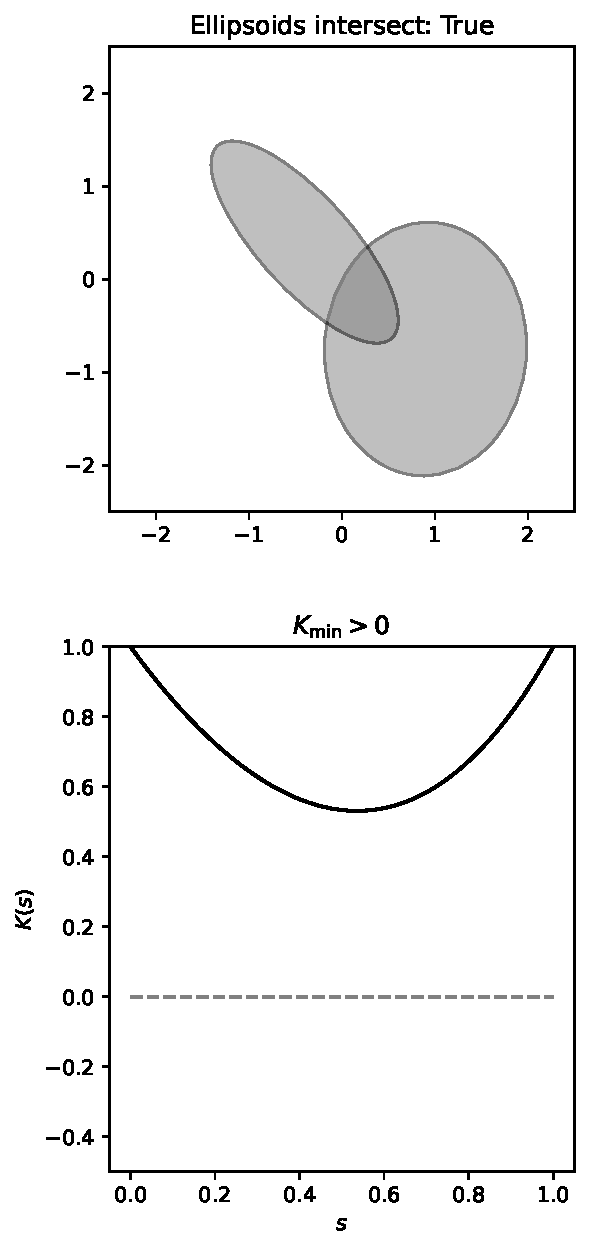
\includegraphics[scale=0.40]{ellipsoids_intersect1.pdf}
	\end{subfigure}
	\begin{subfigure}{0.32\textwidth}
		\centering
		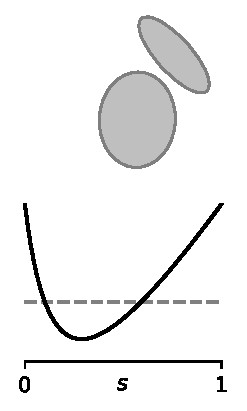
\includegraphics[scale=0.40]{ellipsoids_intersect2.pdf}
	\end{subfigure}
	\caption{The ellipsoids intersect if $K(s) \ge 0$ for all $s \in (0,1)$.
	}
	\label{fig:ellipsoid_intersection_test}
\end{figure}

The function $K(s)$ may be evaluated quickly for many $s$ by pre-computing the solution to the generalized eigenvalue problem
\begin{equation*}
	\spatialcov_1 P = \spatialcov_2 P \Lambda,
\end{equation*}
where $P \in \mathbb{R}^{\gdim \times \gdim}$ is the matrix of generalized eigenvectors (which may be non-orthogonal), and $\Lambda = \diag(\lambda_1,\lambda_2,\dots,\lambda_\gdim)$ is the diagonal matrix of generalized eigenvalues $\lambda_i$. The matrix $P$ simultaneously diagonalizes $\spatialcov_1$ and $\spatialcov_2$, in the sense that $P^T\spatialcov_1 P = \Lambda$, and $P^T\spatialcov_2 P = I$, where $I$ is the $\gdim \times \gdim$ identity matrix. Using this diagonalization, and some algebraic manipulations, we may write $K(s)$ as
\begin{equation}
	\label{eq:Ks_generalized}
	K(s) = 1 - \frac{1}{\tau^2} \sum_{i=1}^\gdim \frac{s(1-s)}{1 + s (\lambda_i - 1)}v_i^2,
\end{equation}
where $v := P^T\left(\spatialmean_1 - \spatialmean_2\right)$. We compute the generalized eigenvalue decomposition of $\spatialcov_1$ and $\spatialcov_2$, then minimize $K(s)$ in the form \eqref{eq:Ks_generalized} on the interval $(0,1)$ using Brent's algorithm \cite{Brent71} (any fast 1 dimensional convex optimization routine may be used). The resulting algorithm for checking whether $E_1$ and $E_2$ intersect is summarized in Algorithm \ref{alg:ellipsoid_intersection_test}.

\begin{algorithm2e}
	\SetAlgoNoLine
	\SetKwInOut{Input}{Input}
	\SetKwInOut{Output}{Output}
	\SetKwProg{Fn}{Function}{}{}
	\Input{Ellipsoid $E_1$ with mean $\spatialmean_1$ and covariance $\spatialcov_1/\tau^2$\\
		Ellipsoid $E_2$ with mean $\spatialmean_2$ and covariance $\spatialcov_2/\tau^2$ 
	}
	
	\Output{Boolean $\text{ellipsoids\_intersect}$ which is true if $E_1 \cap E_2 \neq \{\}$ and false otherwise}
	
	
	Solve generalized eigenvalue problem $\spatialcov_1 P = \spatialcov_2 P \Lambda$
		
	$v \gets P^T\left(\spatialmean_1 - \spatialmean_2\right)$
		
	$\displaystyle K^* \gets \min_{s \in (0,1)}~1 - \frac{1}{\tau^2} \sum_{i=1}^\gdim \frac{s(1-s)}{1 + s (\lambda_i - 1)}v_i^2$
		
	\If{$K^* < 0$}{
			
		$\text{ellipsoids\_intersect} \gets \text{False}$
			
	}
	\Else{
			
		$\text{ellipsoids\_intersect} \gets \text{True}$
			
	}
	\caption{Determining whether two ellipsoids intersect}
	\label{alg:ellipsoid_intersection_test}
\end{algorithm2e}

\subsection{Ellipsoid bounding box test}

One may reduce the average cost of performing ellipsoid intersection tests by first checking whether the coordinate axis aligned bounding boxes for the ellipsoids intersect. If the bounding boxes do not intersect, then the ellipsoids do not intersect, so no further action is necessary. If the bounding boxes intersect, the ellipsoids might intersect, or they might not intersect, so one must perform the complete ellipsoid intersection test described in Section \ref{sec:fast_ellipsoid_intersection_test}.

The smallest coordinate axis aligned box that contains the ellipsoid 
$
E = \{x : (x - \spatialmean)^T \spatialcov^{-1} (x - \spatialmean) \le \tau^2\}
$
is given as follows:
\begin{equation*}
	\prod_{i=1}^\gdim \left[ \spatialmean_i -\tau\sqrt{\Sigma_{ii}}, \spatialmean_i +\tau\sqrt{\Sigma_{ii}} \right],
\end{equation*}
where $\Sigma_{ii}$ is the $i$th diagonal entry of $\Sigma$\footnote{See \url{https://math.stackexchange.com/q/3928964}}. The boxes
\begin{equation*}
	\prod_{i=1}^\gdim \left[a_i^-, a_i^+\right], \quad \text{and} \quad \prod_{i=1}^\gdim \left[b_i^-, b_i^+\right]
\end{equation*}
intersect if and only if $a_i^- \le b_i^+$ and $b_i^- \le a_i^+$ for $i=1,\dots,d$.




\section{Rational positive semi-definite modification}
\label{sec:make_spd}

In many problems of practical interest (e.g., Hessian approximation) $\Aop$ is symmetric positive semi-definite. However, $\mathbf{A}_H$ is generally non-symmetric and indefinite because of approximation error. 
This is undesirable. Symmetry and positive semi-definiteness are important properties which should be preserved if possible. Also, lacking these properties may prevent one from using highly effective algorithms, such as the conjugate gradient method, to perform further useful operations involving $\mathbf{A}_H$.

If $\Aop$ is symmetric, we symmetrize $\mathbf{A}_H$ as follows
\begin{equation*}
\mathbf{A}_H^{\text{sym}} := \frac{1}{2}\left(\mathbf{A}_H + \mathbf{A}_H^T\right).
\end{equation*}
If $\Aop$ is also positive semi-definite, we adapt the high order rational function spectral projection method from \cite[Section 13.8]{HackbuschKress07} to flip (or approximately flip) the negative eigenvalues of $\mathbf{A}_H^{\text{sym}}$ to be positive. In detail, let $\Pi$ be the indicator function for the interval $(a,b)$,
\begin{equation*}
	\Pi(\lambda) = \begin{cases}
		1, & \lambda \in (a,b), \\
		0, & \text{otherwise}.
	\end{cases}
\end{equation*}
Using functional calculus to extend the domain of the function $\Pi$ from scalars to matrices, we define
\begin{equation*}
\mathbf{\Pi} := \Pi(\mathbf{A}_H^{\text{sym}}).
\end{equation*}
The matrix $\mathbf{\Pi}$ is the spectral projector onto the eigenspace of $\mathbf{A}_H^{\text{sym}}$ corresponding to eigenvalues of $\mathbf{A}_H^{\text{sym}}$ that reside in $(a,b)$. If we choose $a < \lambda_\text{min}$ and $b=0$, where $\lambda_\text{min}$ is the smallest eigenvalue of $\mathbf{A}_H^{\text{sym}}$, then $\mathbf{\Pi}$ is the spectral projector onto the eigenspace associated with negative eigenvalues, and $\mathbf{\Pi}\mathbf{A}_H^{\text{sym}}$ is the ``negative component'' of $\mathbf{A}_H^{\text{sym}}$ in which all the negative eigenvalues are the same but all the positive eigenvalues are replaced by zero. Subtracting a negative number from itself twice flips its sign, so the matrix absolute value of $\mathbf{A}_H^{\text{sym}}$ is given by
\begin{equation}
\label{eq:I_Pi_abs}
	|\mathbf{A}_H^{\text{sym}}| = \left(\mathbf{I} - 2\mathbf{\Pi}\right)\mathbf{A}_H^{\text{sym}},
\end{equation}
where $\mathbf{I}$ is the identity matrix of the appropriate size.
By ``matrix absolute value,'' we mean that $|\mathbf{A}_H^{\text{sym}}|$ is the matrix that has the same eigenvectors as $\mathbf{A}_H^{\text{sym}}$, but the eigenvalues of $|\mathbf{A}_H^{\text{sym}}|$ are the absolute values of the eigenvalues of $\mathbf{A}_H^{\text{sym}}$.

\begin{figure}
	\centering
	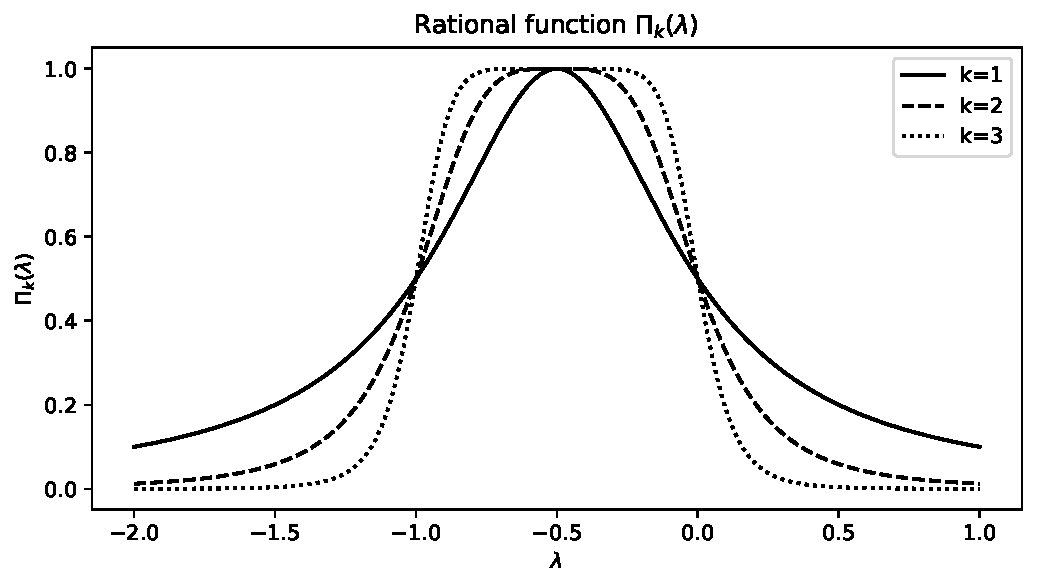
\includegraphics[scale=0.5]{spd_rational_function.pdf}
	\caption{Rational function $\Pi_\ratord(\lambda)$ for $a=-1$, $b=0$, and $\ratord \in \{1,2,3\}$. As $\ratord$ increases, $\Pi_\ratord$ approaches the indicator function for the set $(a,b)$. }
	\label{fig:spd_rat}
\end{figure}

Computing $\mathbf{\Pi}=\Pi(\mathbf{A}_H^{\text{sym}})$ directly is difficult, but we may approximate $\Pi$ by a high order rational function $\Pi_\ratord \approx \Pi$ which is defined as follows:
\begin{equation*}
	 \Pi_\ratord(\lambda) := \frac{1}{1 + T(\lambda)^{2^\ratord} }, \qquad \text{where} \qquad T(\lambda) := \frac{2 \lambda - (b+a)}{b-a}.
\end{equation*}
Here $\ratord$ is a positive integer; the larger $\ratord$ is, the better the approximation $\Pi \approx \Pi_\ratord$. This is illustrated in Figure \ref{fig:spd_rat}. Replacing scalar operations with matrix operations, we have an approximation $\mathbf{\Pi}_\ratord \approx \mathbf{\Pi}$ given by
\begin{equation}
\label{eq:rational343}
\mathbf{\Pi}_\ratord := \Pi_\ratord\left(\mathbf{A}_H^{\text{sym}}\right) = \left(\mathbf{I} + \mathbf{T}^{2^\ratord}\right)^{-1},
\end{equation}
where
\begin{equation*}
\mathbf{T} := T(\mathbf{A}_H^{\text{sym}}) = \left(2 \mathbf{A}_H^{\text{sym}} - (b+a) \mathbf{I}\right)/(b-a).
\end{equation*}
Using $\mathbf{\Pi}_\ratord$ instead of $\mathbf{\Pi}$ in \eqref{eq:I_Pi_abs} allows us to efficiently approximate $|\mathbf{A}_H^{\text{sym}}|$ using H-matrix methods. 
This approximation procedure is as follows. First, we compute $\lambda_\text{min}$ using the Lanczos method, and set $a=\gamma \lambda_\text{min}$ and $b=0$, where $\gamma\ge 1$ is a parameter that must be chosen. 
The method is relatively insensitive to $\gamma$ and numerically we find that the method works well for any $\gamma \in [1,2]$. We use $\gamma=1.5$ in our numerical results. 
Next, we compute $\mathbf{T}$ using fast H-matrix scalar multiplication and addition. We form the $\mathbf{T}^{2^\ratord}$ via repeated squaring, $\mathbf{T}^2 = \mathbf{T} \mathbf{T}$, $\mathbf{T}^4 = \mathbf{T}^2 \mathbf{T}^2$, $\mathbf{T}^8 = \mathbf{T}^4 \mathbf{T}^4$ and so on, where each of these matrix squarings is performed using H-matrix multiplication, which is fast. We recommend using $\ratord=1$ or $2$ (we use $\ratord=1$ in our numerical results). Larger $\ratord$ is unnecessary and may make the method unstable. The approximate spectral projector $\mathbf{\Pi}_\ratord$ is formed from $\mathbf{T}^{2^\ratord}$ per \eqref{eq:rational343}, using fast H-matrix operations to perform the required matrix-matrix addition and matrix inversion. Finally, a positive semi-definite approximation $\mathbf{A}_H^{\text{sym}+}$ of $\mathbf{A}_H^{\text{sym}}$ is formed as
\begin{equation*}
\mathbf{A}_H^{\text{sym}+} := \left(\mathbf{I} - 2\mathbf{\Pi}_\ratord\right)\mathbf{A}_H^{\text{sym}},
\end{equation*}
where fast H-matrix operations are used to perform the necessary matrix-matrix subtraction and multiplication. Note that for any $\ratord \ge 1$, $\Pi_\ratord(\lambda)> 1/2$ for $\lambda \in (a,b)$, so $\mathbf{A}_H^{\text{sym}+}$ is positive semi definite\footnote{Some indefiniteness may be introduced by truncation error in the H-matrix operations, but the negative eigenvalues caused by this truncation error are typically extremely small.}. At the end, $\mathbf{A}_H^{\text{sym}+}$ is symmetrized once again, to correct for any small non-symmetries that are introduced by truncation error in the H-matrix operations. Once constructed, we use the symmetric positive semidefinite matrix $\mathbf{A}_H^{\text{sym}+}$ in place of $\mathbf{A}_H$ in further linear algebra operations.

%\section{Recycling Krylov information via low rank updates}
%\label{sec:recycle_krylov}
%
%In applications, often one wants to use the H-matrix approximation $\mathbf{A}_H$ to build preconditioners for solving a sequence of slowly varying linear systems, where the $k$th linear system has the form
%\begin{equation}
%\label{eq:Ax_equals_b}
%\mathbf{B}^{(k)} \mathbf{u}^{(k)} = \mathbf{f}^{(k)}.
%\end{equation}
%Each of these linear systems is solved using an iterative method. By ``slowly varying,'' we mean that $\mathbf{B}^{(k+1)}$ does not differ much from $\mathbf{B}^{(k)}$. 
%For example, in a Newton-Krylov method for solving an optimization problem, one uses a Krylov method such as conjugate gradient to solve a sequence of systems of the form \eqref{eq:Ax_equals_b}, where $\mathbf{B}^{(k)}$ and $\mathbf{f}^{(k)}$ are the Hessian and the negative gradient of the objective function in the optimization problem, respectively, evaluated at the $k$th Newton iterate. 
%As the optimization solver converges, $\mathbf{B}^{(k)}$ converges to the Hessian at the optimal point, and therefore changes little from one iteration to the next. Since $\mathbf{B}^{(k)}$ varies slowly, it is reasonable to assume that Krylov information about $\mathbf{B}^{(k)}$ can be leveraged to update the preconditioner from $\mathbf{B}^{(k)}$ in order to build a preconditioner for $\mathbf{B}^{(k+1)}$.
%Concretely, let 
%\begin{equation*}
%\mathbf{P}^{(k)} \approx \left(\mathbf{B}^{(k)}\right)^{-1}
%\end{equation*}
%denote a H-matrix preconditioner used to accelerate the solution of \eqref{eq:Ax_equals_b} with an iterative method. The iterative method for solving the $k$th linear system will typically involve, as a sub-problem, applying $\mathbf{B}^{(k)}$ to a collection of vectors $\{\mathbf{x}_i\}_{i=1}^m$, thereby generating vectors $\{\mathbf{y}_i = \mathbf{B}^{(k)} \mathbf{x}_i\}_{i=1}^m$. Instead of rebuilding the H-matrix preconditioner for each successive linear system, we \emph{recycle} the information generated by the iterative method while solving the current linear system, performing a low-rank update to $\mathbf{P}^{(k)}$ to create $\mathbf{P}^{(k+1)}$. To do so, we build on the rank-1 update formulas discussed in \cite[Chapter 6]{NocedalWright99}, which we generalize to many vector ``rank-$m$'' updates. In what follows, let $\mathbf{X}$ and $\mathbf{Y}$ denote the $\fedim \times m$ matrices with columns given by the vectors $\mathbf{x}_i$ and $\mathbf{y}_i$, respectively. The matrix-vector products with $\mathbf{B}^{(k)}$ performed while solving the $k$th linear system may be summarized by the equation:
%\begin{equation*}
%\mathbf{B}^{(k)}\mathbf{X} = \mathbf{Y}.
%\end{equation*}
%To form $\mathbf{P}^{(k+1)}$ from $\mathbf{P}^{(k)}$, one may use one of the following three update formulas:
%\begin{align}
%	\mathbf{P}^{(k+1)} &= \mathbf{P}^{(k)} + \mathbf{R}\left(\mathbf{Y}^T \mathbf{Y}\right)^{-1} \mathbf{Y}^T \label{eq:res_update} \\
%	\mathbf{P}^{(k+1)} &= \mathbf{P}^{(k)} + \mathbf{R} \left(\mathbf{R}^T \mathbf{Y}\right)^{-1} \mathbf{R}^T \label{eq:srk_update} \\
%	\mathbf{P}^{(k+1)} &= \left(\mathbf{I} - \mathbf{X}\boldsymbol{\Theta}\mathbf{Y}^T\right)\mathbf{P}^{(k)}\left(\mathbf{I} - \mathbf{Y}\boldsymbol{\Theta}\mathbf{X}^T\right) + \mathbf{X}\boldsymbol{\Theta}\mathbf{X}^T, \label{eq:dfp_update}
%\end{align}
%where $\mathbf{R} := \mathbf{X}-\mathbf{P}^{(k)}\mathbf{Y}$ and $\boldsymbol{\Theta} := \left(\mathbf{X}^T\mathbf{Y}\right)^{-1}$.
%We note that for all three cases, the update is exact for $\mathbf{B}^{k}$, in the sense that 
%\begin{equation*}
%\mathbf{P}^{(k+1)}\mathbf{Y}=\mathbf{X} = \left(\mathbf{B}^{(k)}\right)^{-1} \mathbf{Y}.
%\end{equation*}
%Because the matrices $\mathbf{B}^{k}$ vary slowly, we expect that $\mathbf{P}^{(k+1)}$ is a good approximation for $\left(\mathbf{B}^{(k+1)}\right)^{-1}$ on the space spanned by the vectors $\mathbf{y}_i$. One should choose which formula to use based on the properties of the matrix $\mathbf{B}^{(k)}$. Formula \eqref{eq:res_update} does not preserve symmetry, and should therefore be used when $\mathbf{B}^{(k)}$ is not symmetric. Formula \eqref{eq:srk_update} preserves symmetry but not positive definiteness, and should therefore be used when $\mathbf{B}^{(k)}$ is symmetric and indefinite. Formula \eqref{eq:dfp_update}, which is used in this paper, preserves both symmetry and positive definiteness, and should therefore be used when $\mathbf{B}^{(k)}$ is symmetric positive definite. Formulas \eqref{eq:res_update} and \eqref{eq:srk_update} perform rank-$m$ updates, while formula \eqref{eq:dfp_update} performs a rank-$2m$ update. 
%We note that when $m=1$, formulas \eqref{eq:srk_update} are \eqref{eq:dfp_update} are known as SR1 (symmetric rank-$1$) and DFP (Davidson-Fletcher-Powell) updates, respectively \cite[Chapter 6]{NocedalWright99}. 

\section*{Acknowledgments}
We thank J.J. Alger, Longfei Gao, Mathew Hu, and Rami Nammour for helpful discussions. We thank Trevor Heise for editing suggestions. We thank Georg Stadler for domain geometry help.

\FloatBarrier

\bibliographystyle{siamplain}
\bibliography{localpsf}

\end{document}
